% Chapter 7

\chapter{Frame semantics for prefixes} % Write in your own chapter title
\label{Chapter7}
%\lhead{Chapter 6. \emph{Frame semantics for prefixes}} 

As I have shown in the previous chapters, Russian verbal \isi{prefixation} is a complex system that cannot be successfully modelled by means of one linguistic layer. In order to simplify individual components of the system and allow for the observed flexibility without massive overgeneration, one needs to coordinate the work of the morphological, syntactic, semantic, and pragmatic representations, as well as describe the interfaces between them. In the fragment I describe here I limit myself to the first three systems, leaving \isi{pragmatic strengthening} at the level of a tentative proposal provided in Chapter~\ref{Chapter6}. Even with this limitation there are not a lot of formalisms that would be suitable for such a representation.

Following \citet{KallmeyerOsswald:12, KallmeyerOsswald:13}, I will adopt a combination of \isi{frame semantics} \citep{Fillmore:82} and Lexicalised Tree Adjoining Grammars\linebreak (\isi{LTAG}, \citealt{JoshiSchabes:97}; \citealt{Frank:92}; \citealt{AbeilleRambow:00}; \citealt{Abeille:02}; \citealt{Frank:02}). This framework has various benefits, such as a transparent syntax-se\-man\-tics interface, numerous factorisation possibilities within the lexicon (especially important for modelling of the derivational morphology), and cognitive plausibility. More information about the advantages of frame-based \isi{LTAG} semantics can be found in \citet{KallmeyerOsswald:13}. 

In this chapter, I concentrate on the semantic side of the analysis and show semantic composition that is triggered by operations at the morphological and syntactic levels. I also provide trees and tree fragments that are associated with the proposed semantic frames, but the presentation is kept on a level suitable also for those readers that are not familiar with \isi{LTAG} and \isi{XMG} 2 \citep{Petitjean:16}. In Chapter~\ref{Chapter8} I will provide more technical details about the syntactic part of the analysis, \isi{metagrammar} decomposition, and specific implementation problems. As for the material that I present in this chapter, the number of decisions motivated by the framework restrictions is small and I discuss all of them. Thus, the proposed frames can be easily adapted to be used within some other framework or even translated into another language of semantic description, e.g. Neo-Davidsonian event representation.

\section{LTAG and frame semantics}
\subsection{TAG}\label{section:tag}
Tree Adjoining Grammar (TAG, \citealt{JoshiSchabes:97}; \citealt{AbeilleRambow:00}) is a tree-rewriting grammar formalism. A TAG consists of a finite set of \textit{elementary trees} with labelled nodes with two operations on them: \textit{substitution} and \textit{adjunction}. 

All elementary trees are either \textit{auxiliary trees} or \textit{initial trees}. An \textit{auxiliary tree} is a tree which has exactly one \textit{foot node} -- a leaf that is marked with an asterisk. Leaf nodes can be labelled with terminals and other nodes are labelled only with non-terminals. The derivation process starts from an \isi{initial tree} and in the final \textit{derived tree} all the leaves must be labelled by terminals.

Substitution allows to replace a non-terminal leaf with a new tree and \isi{adjunction} is used for replacing an \isi{internal} node with an \isi{auxiliary tree}. Adjunction to the node labelled with X is allowed if the root and foot nodes of the adjoining \isi{auxiliary tree} have the same label X. It is also possible to indicate nodes where \isi{adjunction} is obligatory or not allowed and to specify the set of all possible trees for \isi{adjunction}.

Figure \ref{fig:exampletree} shows an example of a derivation: the \isi{initial tree} for \textit{Mary} substitutes into the subject slot of the \isi{elementary tree} for \textit{laughs}, and the \textit{sometimes} \isi{auxiliary tree} for the VP modifier adjoins to the VP node. The result of performing these two operations is shown on the right side of the same figure.

\begin{figure}
% %     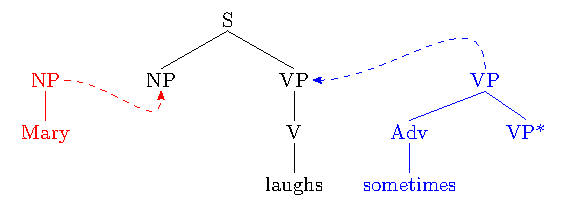
\includegraphics[width=8cm]{treeMaryLaughs.pdf} 
% %     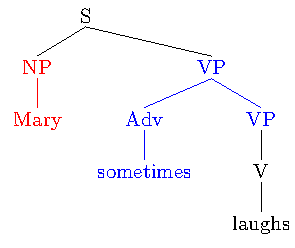
\includegraphics[width=4cm]{derivedTreeMaryLaughs.pdf} 
  \begin{forest}
  [,phantom,s sep=.75cm
    [,phantom,for tree = {red,edge=red}
      [NP,tier=level1,name=NP1 [Mary]]
    ]
    [S
      [NP,tier=level1,name=NP2,inner sep=0pt]
      [VP,name=VP1 [V [laughs]]]
    ]
    [,phantom,for tree = {blue,edge=blue}
      [VP,tier=level1,name=VP2
        [Adv [sometimes]]
        [VP*]
      ]
    ]
    [S
    [NP, for tree={red} [Mary,edge=red]]
    [VP, for tree={blue} 
      [Adv,edge=blue [sometimes,edge=blue]]
      [VP,edge=blue,for tree={black} [V [laughs]]]
    ]
   ]
  ]
  \draw [red, dashed,-{Stealth[]}] (NP1.east) to [in control=+(90:-.5)] (NP2.south);
  \draw [blue, dashed,-{Stealth[]}] (VP2.north) to [out control=+(90:.5),in=360] (VP1.east);
  \end{forest}
    \caption{Example of a TAG derivation}
    \label{fig:exampletree}
\end{figure}

\subsubsection{Feature-structure based TAG} 
Feature-structure based TAG, or FTAG, is a variant of TAG in which elementary trees are enriched with feature structures \citep{Vijay-ShankerJoshi:88}. Using feature structures as non-terminal nodes allows to generalise agreement via underspecification, helps to model \isi{adjunction} constraints and leads to more compact grammars.

For example, \figref{fig:nofstruct} shows the derivation of the sentence \textit{Grammars leak} without feature structures and some trees involved in it (this example, including Figures \ref{fig:nofstruct}--\ref{fig:isleakingresult}, is due to Timm \ia{Lichte, Timm@Lichte, Timm}Lichte). One can see that already such a small piece of derivation contains a lot of redundancy that cannot be avoided if only labelled categories are used. In such a TAG, the following trees have to be kept in the grammar for a regular noun, such as \textit{grammars}: third person singular nominative, third person singular accusative, plural nominative, and plural accusative.

\begin{figure}
% %     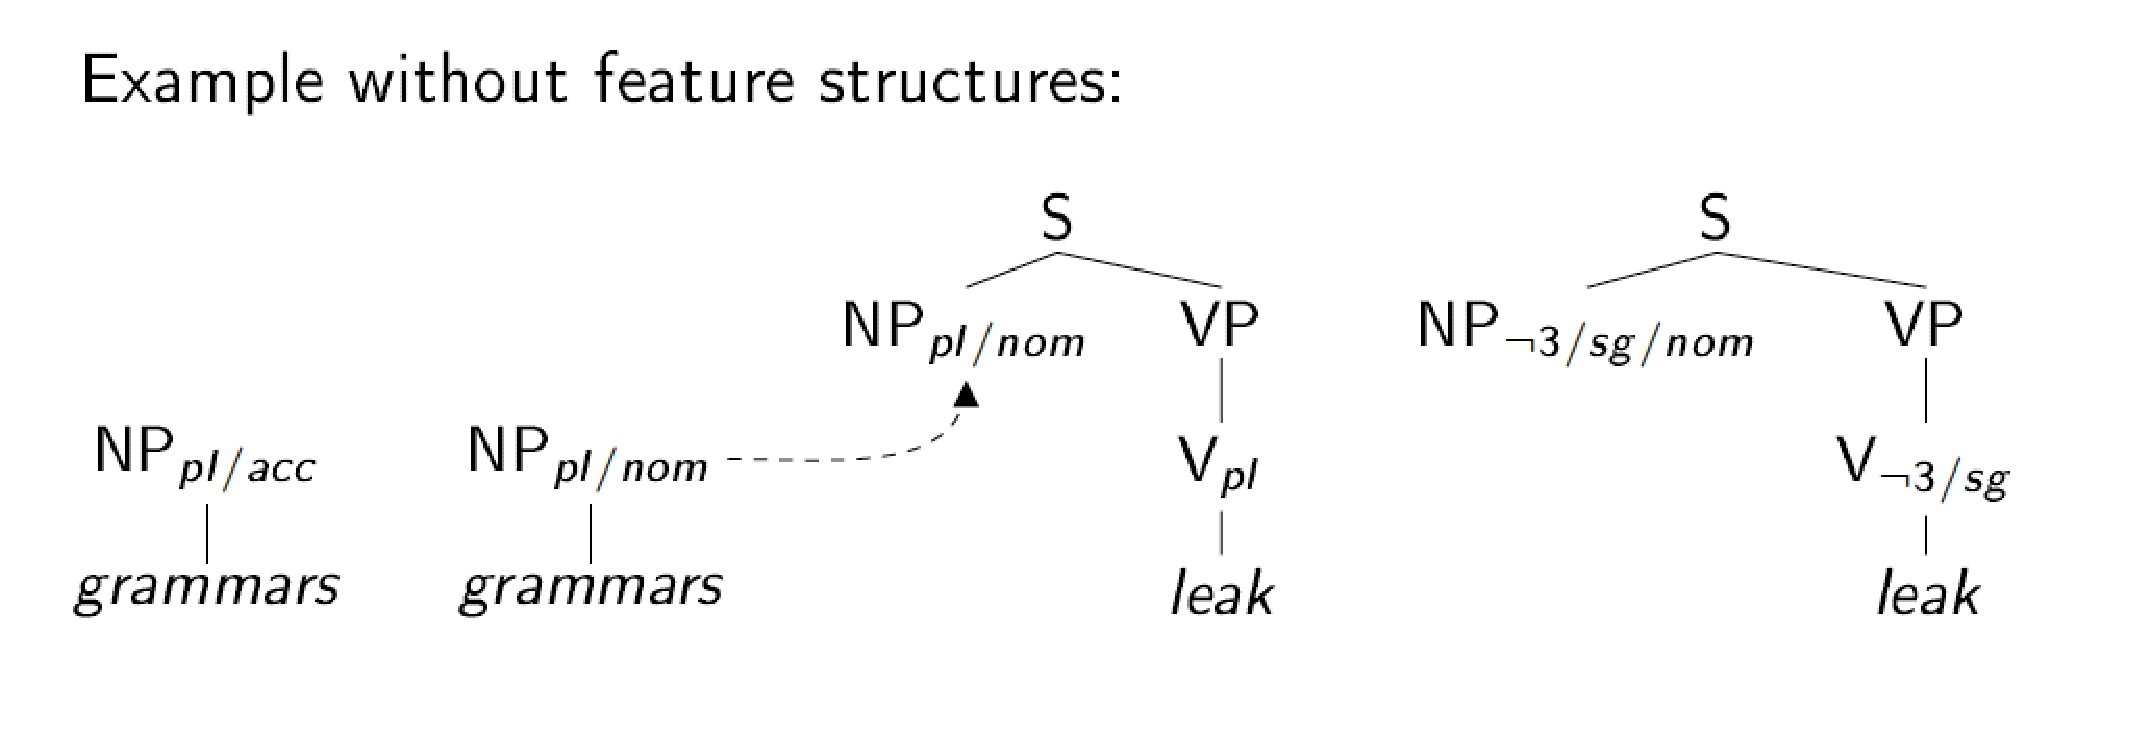
\includegraphics[scale=0.35]{nofstruct.pdf}
\begin{forest}
  [,phantom,for tree={fit=rectangle}
    [,phantom
      [,phantom
       [NP\textsubscript{pl/acc},tier=3 [\textit{grammars},tier=word]]
       [NP\textsubscript{pl/nom},name=NP1,tier=3 [\textit{grammars},tier=word]]
      ]    
    ] 
    [S
      [NP\textsubscript{pl/nom},name=NP2]
      [VP [V\textsubscript{pl},tier=3 [\textit{leak},tier=word]]]
    ]
    [S
      [NP\textsubscript{¬3/sg/nom}]
      [VP [V\textsubscript{¬3/sg},tier=3 [\textit{leak},tier=word]]]
    ]
  ]
\draw [dashed,-{Triangle[]}] (NP1.east) to[bend right] (NP2.south);
\end{forest}
    \caption{Example of a derivation for \textit{Grammars leak} without feature structures  \label{fig:nofstruct}}
\end{figure}

If feature structures are used, the example described above looks as shown on \figref{fig:grleaksubst}. In this case only two entries for the noun \textit{grammar} must be kept in the lexicon: one for the single form \textit{grammar} and one for the plural form \textit{grammars}. Case can remain underspecified, as it does not influence the surface form of the noun.

\begin{figure}
% %     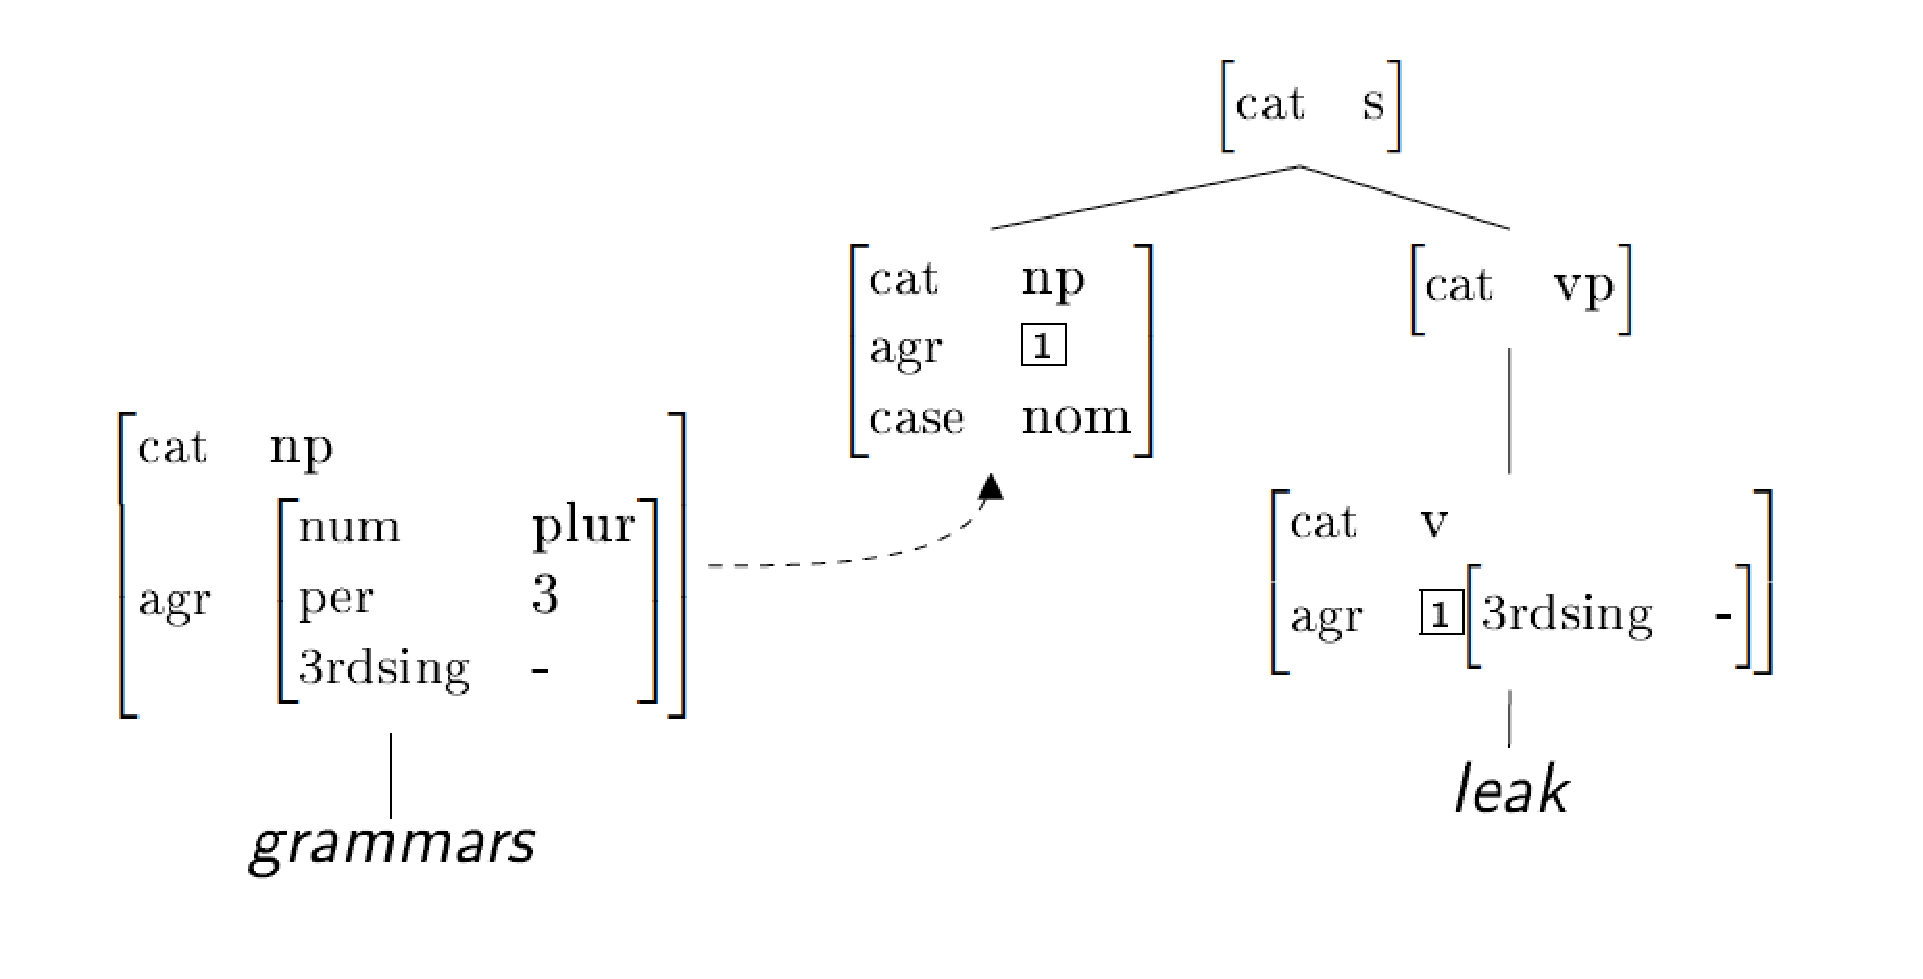
\includegraphics[scale=0.35]{grammarsleak.pdf}
    \avmsetup{style=plain}
\begin{forest}
  [,phantom,fit=rectangle
    [,phantom
     [,phantom
       [\avm{
         [cat & np\\
          agr & [ num & plur \\
                  per & 3\\
                  3rdsing & \textminus]
         ]
       },name=avm1
         [\textit{grammars},tier=word]
       ]
     ]
    ]
    [\avm{[cat & s]}
     [\avm{
       [cat & np\\
        agr & \1\\
        case & nom]
     },name=avm2]
     [\avm{[cat & vp]}
       [\avm{
         [cat & v \\
          agr & \1[3rdsing & \textminus]]
       }
         [\textit{leak},tier=word]
       ]
     ]
    ]
  ]
  \draw[dashed,-{Triangle[]}] (avm1.east) to[out=0,in=270] (avm2.south);
\end{forest}
    \caption{Example of a derivation for \textit{``Grammars leak"} with feature structures \label{fig:grleaksubst}}
\end{figure}

However, when \isi{adjunction} is performed, the \isi{adjunction} site is practically split in two. In this case, feature structures must be also split. Such a split has been proposed by \citet{Vijay-ShankerJoshi:88}. The idea behind it is that top features should show ``what the node represents in the surrounding structure" and bottom features should show ``what the tree below the node represents".

As a result, in an FTAG all the nodes have a top feature structure and, furthermore, all nodes except \isi{substitution} nodes have a bottom feature structure. Feature \isi{unification} applies during the derivation process when \isi{adjunction} and \isi{substitution} take place and is performed according to the following rules:
\begin{itemize}
\item when \isi{substitution} takes place, the top of the root of the rewriting tree unifies with the top of the \isi{substitution} node;
\item when \isi{adjunction} takes place, the top of the root of the rewriting tree unifies with the top of the \isi{adjunction} site, and the bottom of the foot of the rewriting tree unifies with the bottom of the \isi{adjunction} site (as illustrated by Figures~\ref{fig:isleaking} and~\ref{fig:isleakingresult}).
\end{itemize}

\begin{figure}\small
% %     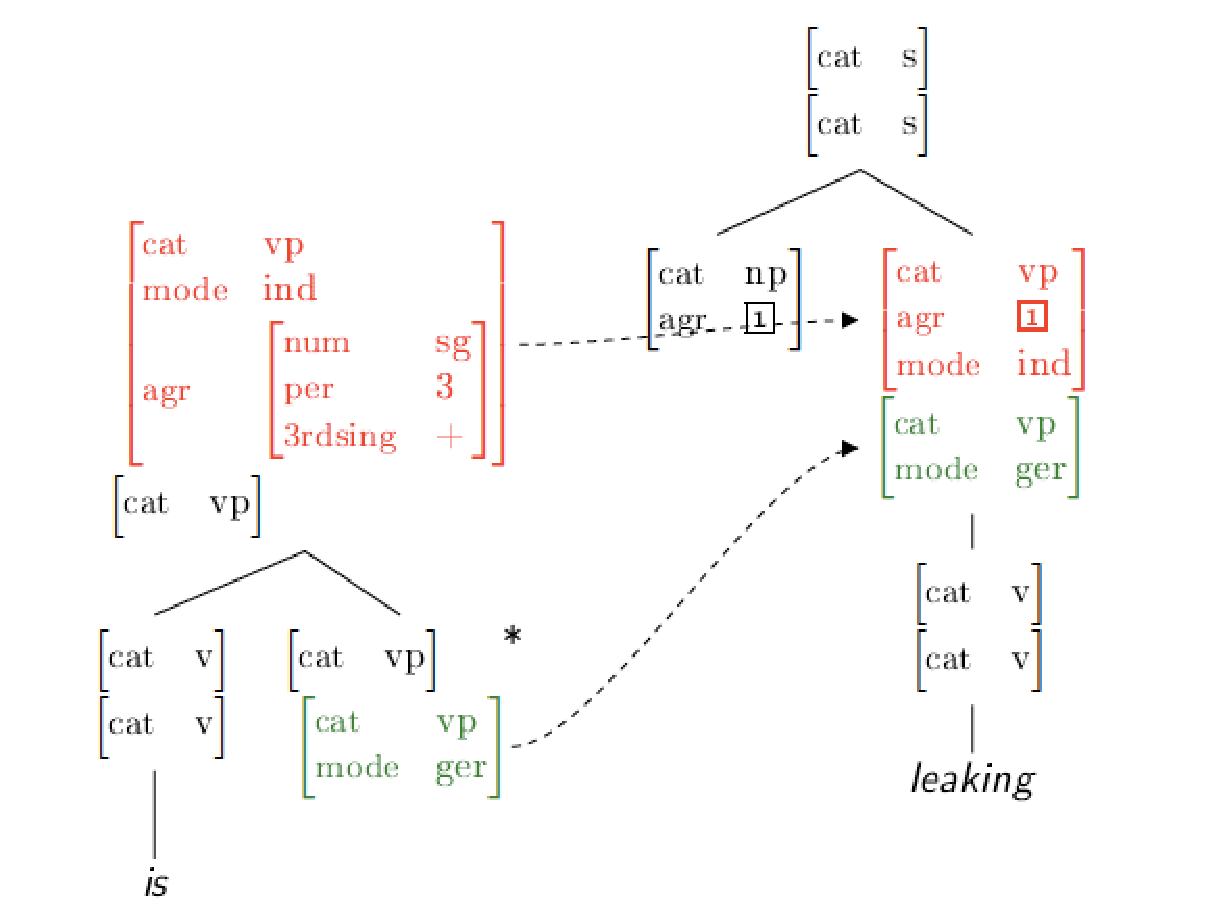
\includegraphics[scale=0.5]{isleaking.pdf}
  \avmsetup{style=plain}
  \begin{forest}
[,phantom,for tree={fit=rectangle}
  [,phantom
    [,phantom
     [{\color{lsRed}\avm{
     [cat & vp\\
      mode & ind\\
      agr  & [num & sg\\
              per & 3\\
              3rdsing & +]]
    }}\smallskip\\
    \avm{[cat & vp]},name=avm1
    [\avm{[cat & v]}\smallskip\\
     \avm{[cat & v]}
      [\textit{is},tier=word] 
    ]
    [\avm{[cat & vp]}\smallskip\\
     {\color{lsRichGreen}\avm{
       [cat & vp\\
        mode & ger]
     }},name=avm2
    ]
    ]
   ]  
  ]
  [\avm{[cat & s]}\smallskip\\
   \avm{[cat & s]}\smallskip\\
     [\avm{[cat & np\\
            agr & \1]}]
     [{\color{lsRed}\avm{
       [cat & vp\\
        agr & \1\\
        mode & ind]
     }}\smallskip\\
      {\color{lsRichGreen}\avm{
        [cat & vp\\
         mode & ger]
      }},name=avm3
       [\avm{[cat & v]}\smallskip\\
        \avm{[cat & v]}
          [\textit{leaking},tier=word]
        ]     
     ]
  ]
]
\draw[dashed,-{Triangle[]}] (avm1) to[out=345,in=210] (avm3.170);
\draw[dashed,-{Triangle[]}] (avm2) to[out=345,in=210] (avm3);
  \end{forest}
    \caption{Adjunction of \textit{is} into the tree for \textit{leaking}     \label{fig:isleaking}}
\end{figure}

\begin{figure}\small
% %     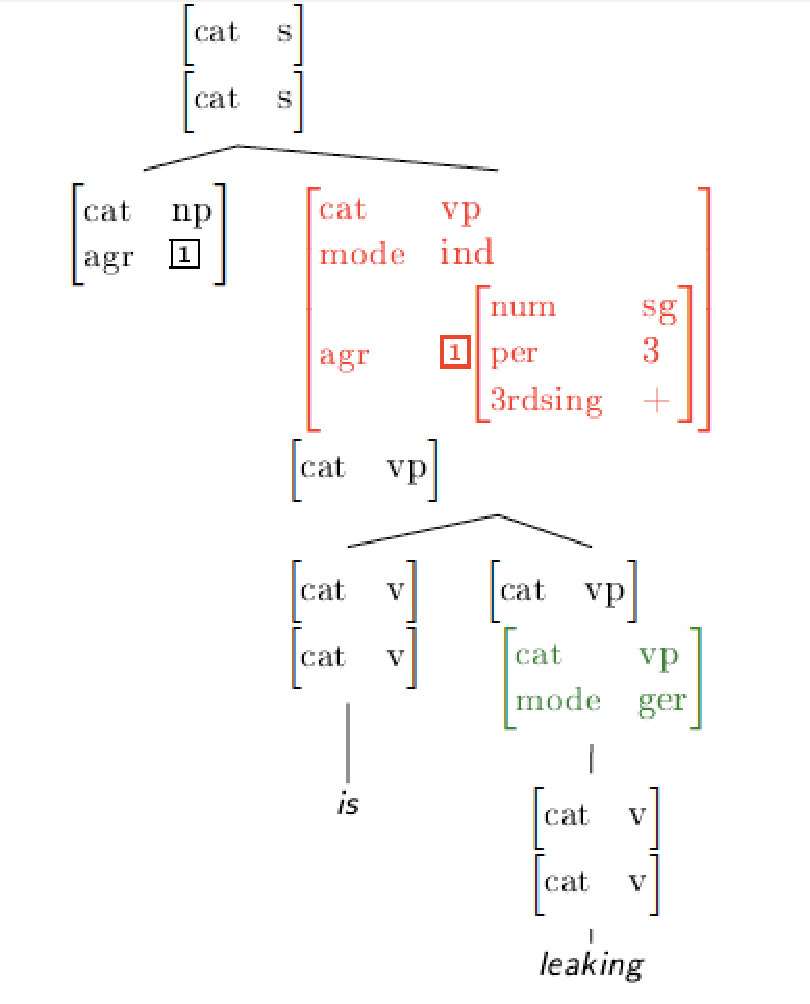
\includegraphics[scale=0.5]{isleakingresult.pdf}
    \avmsetup{style=plain}
    \begin{forest}
    [\avm{[cat & s]}\smallskip\\
     \avm{[cat & s]}
      [\avm{[cat & np \\ agr & \1]}]
      [{\color{lsRed}\avm{
        [ cat & vp\\
          mode & ind\\
          agr & \1 [num & sg\\
                    per & 3\\
                    3rdsing & +]
        ]
        }}\smallskip\\
        \avm{[cat & vp]}
          [\avm{[cat & v]}\smallskip\\
           \avm{[cat & v]}
             [\textit{is}]
          ]
          [\avm{[cat & vp]}\smallskip\\
           {\color{lsRichGreen}
            \avm{[cat & vp\\mode & ger]}
           }
           [
             \avm{[cat & v]}\smallskip\\
             \avm{[cat & v]}
             [\textit{leaking}]
           ]
          ]
       ]
    ]
    \end{forest}
    \caption{Adjunction of \textit{is} into the tree for \textit{leaking}: result \label{fig:isleakingresult}}
\end{figure}

In the final \isi{derived tree}, top and bottom feature structures unify for all nodes. Feature structures used in an FTAG are allowed to have re-entrancies, but the same attribute should not occur on the path more than once. Due to the extended domain of locality of TAGs, nodes within one \isi{elementary tree} can share features, allowing to express constraints among dependent nodes easily. On the other hand, the feature structures of FTAG belong to a finite set and thus do not add expressive power, so FTAG and TAG are weakly equivalent.

%To sum up, FTAG is used instead of the simple TAG because feature structures as nodes allow to abstract away from agreement properties by underspecification, which leads to the fact that linguistic generalizations can be expressed more conveniently. Moreover, a split into top and down features provide a convenient mechanism for encoding \isi{adjunction} constraints, as was illustrated by \figref{fig:isleaking} and \ref{fig:isleakingresult}. Another important fact is that

\subsubsection{Lexicalised TAG} 
\citet{Abeille:02} and \cite{Frank:02} formulate principles that specify how TAG elementary trees should look like if they are used to model natural languages. First, each \isi{elementary tree} must have at least one non-empty lexical item. This item is called \textit{lexical anchor}. When all the elementary trees satisfy this condition, a TAG is called \textit{lexicalised TAG,} or \isi{LTAG}. This property has been argued to be a reasonable requirement with respect to modelling of natural languages. On the computational side it reduces the parsing time. 

The second important principle for a natural language TAG is called \textit{theta-criterion for TAG} \citep{Frank:92}, or \textit{\isi{elementary tree} minimality}. It requires that every \isi{elementary tree} with a predicate as a \isi{lexical anchor} must contain slots (\isi{substitution} nodes or foot nodes) for all arguments of this predicate (including the subject) and for nothing else. Nominal arguments are usually represented as \isi{substitution} nodes, whereas sentential arguments are often realised by foot nodes in order to allow long-\isi{distance} dependency constructions through \isi{adjunction}  \citep{Kroch:89, Frank:02}.

%\ex.\label{ex:extraction} Whom does John think that Mary hates?

As I have already mentioned, there are several levels of factorisation of the \isi{LTAG} lexicon. The first step is the separation of \isi{lexical anchors} and tree templates (unanchored elementary trees). As a second step, the set of elementary trees is organised into tree families. Each tree family represents all possible realisations of one subcategorisation frame: e.g., there is a tree family for \isi{transitive verbs} (this means \isi{transitive verbs} should be used as \isi{lexical anchors}, i.e. fill the node marked with a diamond). This tree family contains patterns as shown on \figref{fig:treefamily}: canonical position, argument extraction, realisation in combination with a passive verb form, among others.

\begin{figure}
% \begin{tabular}{l l l}
% 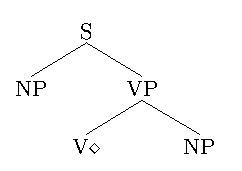
\includegraphics[scale=0.9]{TransVerb.pdf}
% &
% 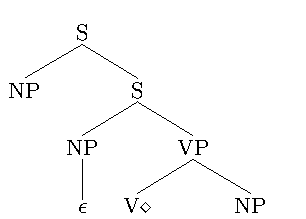
\includegraphics[scale=0.9]{TransVerb2.pdf}
% &
% 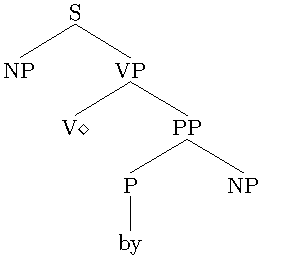
\includegraphics[scale=0.9]{TransVerb3.pdf}
% \end{tabular}
\begin{forest}
[S
 [NP]
 [VP
   [V◇]
   [NP]
 ]
]
\end{forest}\hfill
\begin{forest}
[S
  [NP]
  [S
   [NP [$\epsilon$,no edge,tier=word]]
   [VP [V◇,tier=word] [NP,tier=word]]
  ]
]
\end{forest}\hfill
\begin{forest}
[S
  [NP]
  [VP
    [V◇]
    [PP
      [P [by]]
      [NP]
    ]
  ]
]
\end{forest}\hfill
\caption{Some elemantary trees from the transitive verb tree family\label{fig:treefamily}}
\end{figure}

The next factorisation level is the decomposition of tree templates into tree fragments, that is done using a \textit{metagrammar} description \citep{Candito:99, CrabbeDuchier:04, Crabbe:13}. The idea of the \isi{metagrammar} is to define tree fragments that can be used in different tree templates and tree families. These tree fragments are minimal models of a constraint system that operates in terms of category assignments and dominance and precedence relations. Such system allows for a compact linguistic description that captures generalisations. 

The level of the \isi{metagrammar} is well-suited for capturing derivational morphology processes: it allows for a general description of derivational patterns that can be accompanied by a change of the \isi{argument structure}. I will talk about the technical details of the \isi{metagrammar} description in Chapter~\ref{Chapter8}. As for now, it is important to know that frames shown in what follows belong to four different description levels: 
\begin{enumerate}
\item frames for the prefixes, frames used for coercion, and \isi{dimension constructors} accompany special tree fragments that are described in the \isi{metagrammar}; 
\item frames for the verbs are stored in the dictionary; 
\item frames that represent the result of combining the frame for the \isi{derivational base} and the prefix frame are obtained when the unanchored trees produced by the \isi{metagrammar} description get anchored; 
\item frames that represent the semantics of a verbal phrase are obtained on parallel with the syntactic parsing.
\end{enumerate}

\subsection{Frame Semantics}
The idea of using frame representations in linguistic semantics and cognitive
psychology has been put forward by \citet{Fillmore:82} and
\citet{Barsalou:92}, among others. A widescale realisation of this idea is the Berkeley FrameNet project \citep{Fillmore:03}. The goal of this project is to describe a huge variety of situations by basic role frames that represent the type of the situation and the semantic roles of its participants. One issue that FrameNet does not address is modelling \isi{compositional semantics}: the frames used in the project are static and do not interact with each other. In order to widen the area where frames could be used, a number of studies that offer further formalisation of the frame theory has been conducted in the last years (\citealt{Petersen:07, PetersenOsswald:10, KallmeyerOsswald:12, KallmeyerOsswald:13, KallmeyerOsswaldPogodalla:15, Loebner:2014}, among other).

The main ideas that motivate the use of frames as a general semantic and conceptual representation format can be summarised as follows (cf.\ \citealt{Loebner:2014}):

\begin{itemize}
\item conceptual-semantic entities can be described by types and
attributes;
\item attributes are functional relations, i.e., each attribute assigns a unique
value to its carrier;
\item attribute values can be also characterised by types and attributes (recursion);
\item attribute values may be connected by additional relational constraints \citep{Barsalou:92} such as \isi{spatial} configurations or ordering relations.
\end{itemize}

These ideas are formalised in \citet{KallmeyerOsswald:13} who define frames
as \emph{base-labelled feature structures with types and relations}.
Frames in the sense of \citet{KallmeyerOsswald:13} are finite relational structures in which attributes correspond to functional relations. The members of the underlying set are referred to as the \emph{nodes} of the frame. An important restriction is that any frame must have a \emph{functional
backbone}. This means that every node has to be accessible via attributes
from at least one of the \emph{base nodes}: nodes that carry \emph{base labels}. Importantly, feature structures may have multiple base nodes. In such a case often some nodes that are accessible from different base nodes are connected by a relation.

Base labels serve as unique identifiers, that is, a given base label cannot be assigned to more than one node. Due to the functional backbone requirement, every node of the frame can be addressed by a base label
plus a (possibly empty) finite sequence of attributes.
The middle column of \figref{fig-frame-example} (this figure and \figref{fig-frame-example-II} are provided by Rainer Osswald) illustrates this fact
for the frame depicted on the left of the figure, where circles
represent nodes, the bold-face letters \fsbase{b} and \fsbase{c} are base
labels, labels of solid arrows stand for attributes, labels of dotted arrow
indicated (binary) relations, and the symbols $s$ and $t$ are types.\largerpage

\begin{figure}
\fbox{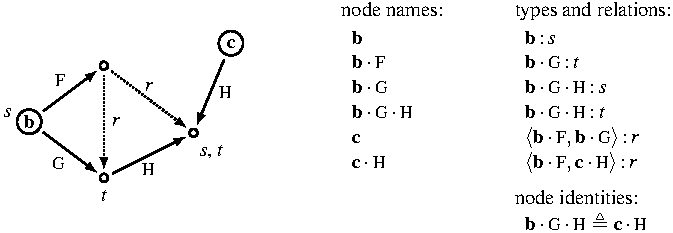
\includegraphics[width=\textwidth - 3\fboxsep]{fig-frame-example}}%
\caption{Example of a base-labelled feature structure with types and relations\label{fig-frame-example}}
\end{figure}

As the example on \figref{fig-frame-example} reveals, a node can have more than one type. The special property of the type system used in frame theory as it is presented in \citealt{KallmeyerOsswald:13} is that type \isi{conjunction} is always possible unless it violates explicitly stated incompatibility constraints. We will return to the discussion of the \isi{type hierarchy} in Section~\ref{section:types}.

Frames as attribute-value descriptions can be reformulated in terms of first-order predicate logic and thus related to other semantic representation formats, such as Neo-Davidsonian event semantics. In such a reformulation (fully described in \citealt[Section~3.3.3]{KallmeyerOsswald:13}), types and base
labels are regarded as one-place predicates, attributes as two-place predicates, and relation symbols as $n$-place predicates with $n>1$.
In addition, attributes are required to be functional and \isi{base labels} must
not denote more than one node;
that is, the following two axioms are assumed to hold for all
attributes $f$ and \isi{base labels} $l$:

\ex.\label{ex.fun-axioms}
$\every u\every v\every w(f(u,v)\und f(u,w)\ifthen v=w)$
\quad and \quad
$\every u\every v(l(u)\und l(v)\ifthen u=v)$
%\a.\label{ex.funrel-axiom}
%$\every u\every v\every w(f(u,v)\und f(u,w)\ifthen v=w)$
%\b.\label{ex.funbase-axiom}
%$\every u\every v(l(u)\und l(v)\ifthen u=v)$

The frame shown on \figref{fig-frame-example} can be viewed
as a \emph{model} of the formula shown on the upper left of \figref{fig-frame-example-II} (in the sense of predicate logic). This model also satisfies the formulas given in \ref{ex.fun-axioms}. In what follows I will use frames in form of attribute-value matrices, like the frame shown on the right side of \figref{fig-frame-example-II}.

\begin{figure}
\fbox{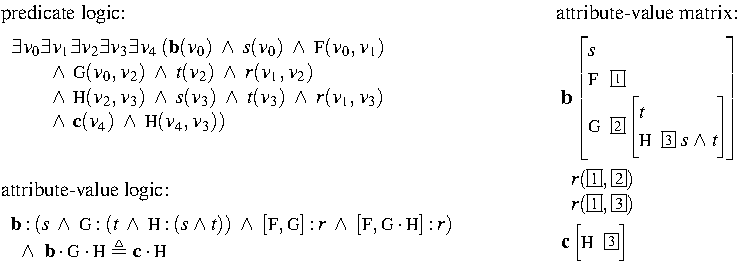
\includegraphics[width=\textwidth - 3\fboxsep]{fig-frame-example-II}}%
\caption{Alternative ways of specifying the frame on the left side of
\figref{fig-frame-example}\label{fig-frame-example-II}}
\end{figure}

For the purposes of a \isi{metagrammar} specification we need another way of description of frames: attribute-value logic that is defined in \citealt[Section~3.3.2]{KallmeyerOsswald:13}. It is constructed as a language of general attribute-value descriptions and then complemented by \isi{base labels}.\pagebreak

The primitive general attribute-value descriptions over a signature $\langle A, T, R \rangle$ are expressions of the form: \[t, r, p : t, p \doteq q, p \triangleq q, (p_1, \ldots , p_n) : r\] and \[\langle p_1, \ldots , p_n \rangle : r \text{, with } p, p_i, q \in A^*, t \in T \text{, and }r \in R\text{.}\] For a feature structure $F = \langle V, \delta, \tau, \pi \rangle$ over a signature $\langle A, T, R \rangle$ with $v,w, v_i \in V$ the satisfaction relation $\models$ between attribute-value descriptions and nodes/node tuples of $F$ is defined as shown in \ref{def:satisfaction} (Def.~3 in \citealt{KallmeyerOsswald:13}).

\ex.\label{def:satisfaction}
\begin{tabular}[t]{@{}llll@{}}
a. & $v \models t$   & iff &  $v \in \tau (t)$\\
b. & $\langle v_1, \ldots , v_n \rangle \models r$   & iff &  $\langle v_1, \ldots , v_n \rangle \in \rho (t)$\\
c. & $v \models p : t$   & iff &  $\delta (v, p) \models t$\\
d. & $v \models p \doteq q$   & iff &  $\delta (v, p) = \delta (v, q)$\\
e. & $\langle v, w \rangle \models p \triangleq q$   & iff &  $\delta (v, p) = \delta (w, q)$\\
f. & $v \models (p_1, \ldots , p_n ) : r$   & iff &  $\langle \delta (v, p_1), \ldots , \delta (v, p_n) \rangle \models r$\\
g. & $\langle v_1, \ldots , v_n \rangle \models \langle p_1, \ldots , p_n \rangle : r$   & iff &  $\langle \delta (v, p_1), \ldots , \delta (v, p_n) \rangle \models r$
\end{tabular}

Labelled attribute-value descriptions are of the form $l \cdot \phi, l \cdot p \triangleq k \cdot q$, and $\langle l_1 \cdot p_1, \ldots , l_n \cdot p_n \rangle : r$, with $k, l, l_i \in B$. The satisfaction conditions are listed in \ref{def:labelled} (Def.~4 in \citealt{KallmeyerOsswald:13}).

\ex.\label{def:labelled}
\begin{tabular}[t]{@{}llll@{}}
a. & $\langle F, \beta \rangle \models l \cdot \phi$   & iff &  $\beta (l) \models \phi $\\
b. & $\langle F, \beta \rangle \models l \cdot p \triangleq k \cdot q $   & iff &  $\langle \beta (l), \beta (k) \rangle \models p \triangleq q$\\
c. & $\langle F, \beta \rangle \models \langle l_1 \cdot p_1, \ldots l_n \cdot p_n \rangle : r$   & iff &  $\langle \delta (\beta (l_1), p_1), \ldots \delta (\beta (l_n), p_n) \rangle \models r $\\
\end{tabular}

Labelled descriptions are allowed to be combined with Boolean operators. The attribute-value matrix shown on the right side of \figref{fig-frame-example-II} can be regarded as a normal form of the \isi{attribute-value description} given at the bottom of the left side of the same figure. 

\subsection{Combining TAG and frame semantics}
There is a number of properties that make \isi{LTAG} a good candidate for a combination with a frame-based \isi{compositional semantics}. Two properties are especially important in this respect: the combination of an extended domain of locality and the fact that elementary trees are lexicalised and contain slots for all the arguments of the respective predicate. This allows to link semantic representations directly to the argument slots. It is also convenient that no structural parallelism is required between the syntactic and semantic representations, as argument linking is explicit. The combination of an \isi{LTAG} and \isi{frame semantics} has been introduced in \cite{KallmeyerOsswald:12} and the most extensive description so far has been provided in \citet[Section~4.1]{KallmeyerOsswald:13}.

In the approach proposed in \cite{KallmeyerOsswald:13} that I adopt here, a single semantic representation (a semantic frame in this case) is linked to the entire \isi{elementary tree}. When an \isi{elementary tree} is coupled with a semantic frame, syntactic arguments can be directly linked to their counterpart in the semantics. (Similar approaches with different semantic representation frameworks were introduced earlier in \cite{GardentKallmeyer:03} and \cite{KallmeyerRomero:08}.) Semantic composition is then modelled by \isi{unification}, which is a result of performing adjunctions and substitutions. \figref{fig:examplesemantic} provides a simple illustration of the syntactic and semantic composition. The feature I on the nodes is a \isi{syntax-semantics interface} feature. It stands for ``individual'' and is used for argument linking. In this example, substitutions trigger unifications between the nodes \svar{1} and \btag{g} and  between the nodes \svar{2} and \btag{h}. This leads to the correct insertion of the argument frames into the frame of \textit{loves}. The resulting \isi{frame representation} is shown on \figref{frame:love}.

\begin{figure}
% %     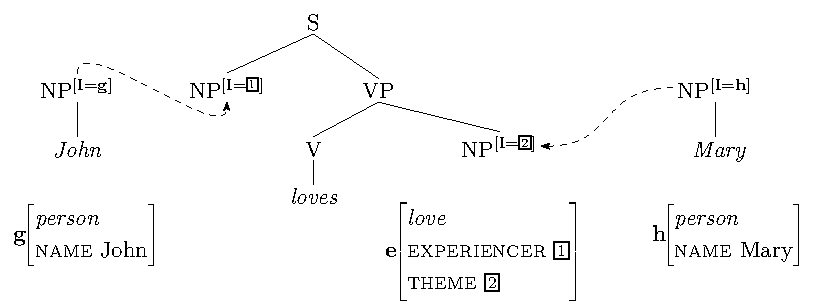
\includegraphics[scale=0.8]{treeJohnLovesMary.pdf} 
\begin{forest}
[,phantom,for tree={fit=rectangle}
 [,phantom
   [NP\textsuperscript{[I=\textbf{g}]},tier=cat,name=NP1
     [\textit{John}\\
      \avm{\textbf{g}[\type*{person}\\name & John]},tier=word
     ]
   ]
 ]
 [S
   [NP\textsuperscript{[I=\avm{\1}]},tier=cat,name=NP2]
   [VP
     [V [\textit{loves}\\
         \avm{\textbf{e}[\type*{love}\\
                         experiencer & \1\\
                         theme & \2]},tier=word
     ]]
     [NP\textsuperscript{[I=\avm{\2}]},name=NP3]
   ]
 ]
 [,phantom
   [NP\textsuperscript{[I=\textbf{h}]},tier=cat,name=NP4
     [\textit{Mary}\\
     \avm{\textbf{h}[\type*{person}\\name & Mary]},tier=word
     ]
   ]
 ]
]
\draw[dashed,-{Triangle[]}] (NP1) to[out=90,in=270] (NP2);
\draw[dashed,-{Triangle[]}] (NP4) to[out=180,in=360] (NP3);
\end{forest}
    \caption{Syntactic and semantic composition of \textit{John loves Mary}\label{fig:examplesemantic}}
\end{figure}

\begin{figure}
\avm{
\btag{e} [\type*{love}
	   \EXP &  \1 \btag{g} [\type*{person}
	   		\NAME & John ]\\
      \THEME &  \2 \btag{h} [\type*{person}
	   		\NAME & Mary ]
]
}
\caption{Result of frame unifications shown on \figref{fig:examplesemantic} \label{frame:love}}
\end{figure}


\subsection{Type hierarchy}\label{section:types}
The \isi{type hierarchy} is one of the crucial elements of the analysis, as it is the main mechanism of blocking derivations. Since the number of \isi{syntactic restrictions} I use is very limited, many derivations will be filtered out by the \isi{semantic constraints}. For this, there are two main mechanisms: \isi{unification failure} (type incompatibility or conflicting attribute values) and constraint failure (requirement for the two values to be in a specific relation is not satisfied). 

As I have already mentioned above, any two types can be unified unless there is an explicit constraint that prohibits it. Due to this, adding new types to the \isi{type hierarchy} is an operation that in most cases can be performed very fast: usually all that one has to do is to specify one or more supertypes of the new type. I will use the term \textit{subtype of type x} to refer to a type that is ordered under the type \textit{x}. Such hierarchy architecture leads to a large number of connections (e.g.\ in \isi{comparison} with a \isi{type hierarchy} in HPSG, \citealt{PollardSag:94}), so I will not show the full hierarchy of types used in this chapter, and mostly talk about the relevant restrictive statements (incompatibility of certain types).

The list of types I use for the frames in this chapter and for the implementation to follow can be divided into three major categories (three subtypes of the type \textit{root}): \textit{entity, event,} and \textit{scale.} Among these, \textit{entity} is the only type that is not compatible with the other two. It has subtypes \textit{object} and \textit{person}, that in turn have subtypes and are not compatible with each other. As I do not aim at constructing a large ontology, I use trivial object types and assume that they cannot be unified.

The \isi{part of the hierarchy} that is more interesting for the current analysis concerns the subtypes of events and \isi{scales}. Let us start with events. I will be using the following types of events (not compatible with each other): \textit{process, state,} and \textit{transition.} These types can be combined with the event types \textit{bounded-event} and \textit{iteration}. Such classification covers Vendler's \citep{Vendler:67} four-way distinction between states, activities (\textit{process} here), accomplishments (\textit{process $\wedge$ bounded-event} here), and achievements (\textit{transition}). What is not built into the type system is the distinction between dynamic and static states, that is used, e.g., by \citet{Bach:86}. The rest of the classification proposed in \citealt{Bach:86} is effortlessly expressed: process has the same name, protracted event is a \textit{process $\wedge$ bounded-event}, happening is \textit{transition}, and culmination is \textit{transition} that has a \isi{preparatory phase}. These types may have subtypes: e.g., \textit{translocation} and \textit{change-of-state} are subtypes of a process.

The last and most important part of \isi{type hierarchy} for this work is the domain of \isi{scales}. The main subtypes of the type \textit{scale} are \textit{\isi{closed-scale}, \isi{one-marked-point}, proper-scale, measure-of-change, cardinality}, and \textit{property}. These six types come in three groups such that the subtypes of one group are not compatible with each other. The first group is constituted by the types \textit{closed-scale} and \textit{one-marked-point}, that refer to the presence of end points and are not compatible with each other. To the second group belong the types \textit{measure-of-change} and \textit{proper-scale}. They describe how the scale is organised: in case of a \textit{proper-scale,} for each point of the scale there must be an event stage that is characterised exactly by this point. The \textit{measure-of-change} scale type does not have such requirements: as long as the initial and the final stage of the event are associated with particular scale values, any intermediate stages are allowed. The last group is formed by the \textit{cardinality} and \textit{property-scale} types that refer to the dimension and not to the structure of the scale. Subtypes of the \textit{property-scale} type (such as \textit{colour, temperature, length, amount} etc.) are not compatible with each other. The \textit{cardinality} type of the scale allows to talk about iterated events.

A special case is the case of \isi{conjunction} of the types \textit{event} and \textit{scale}. The idea that underlies it is that events may be conceived as carrying a scalar structure by themselves. One can talk about event \emph{stages} that hold at different moments in the course of the event. Thus, stages are instantaneous situations that are ordered by temporal precedence and can be used to talk about time in connection to the event but without relating this to other events in the world or any kind of a global time representation. For more details, see \citet{ZinovaOsswald:paper}.\footnote{Note that it is not necessary to represent time \isi{scales} this way, more explicit representations will also be compatible with the frames proposed in this chapter.}
%*Here has to come a picture of the relevant \isi{part of the hierarchy}*

Now that all the parts needed for the analysis are introduced, let us move to the sections that are dedicated to the particular prefixes.

\section{Frame semantics for the prefix \textit{za-}}\label{section:frame:za}
In this section I propose the frame semantic representation for the \isi{inchoative} interpretation of the prefix \Prefix{za-} and show how this prefix combines with a verb. To start, let us recall the conclusions that I have made about the prefix \Prefix{za-} (in particular about its \isi{inchoative} interpretation) in Chapter~\ref{Chapter5} by further developing the ideas of \citet{Braginsky:08} and \citet{Kagan:book}. First, I proposed that the \isi{inchoative} interpretation of the prefix is only possible when the \isi{derivational base} does not contain any explicit \isi{scales} except for the \isi{time scale} in their semantic representation. Second, I offered the following description of the semantic contribution of the prefix \Prefix{za-} under \isi{inchoative} interpretation: when the prefix is attached, it relates the initial stage of the event to the state of the absence and the final stage of the event to the state of the presence of the activity denoted by the \isi{derivational base}.

There are two ways in which the proposed requirement regarding the scale type can be connected with the semantic change caused by the prefix attachment: a \textit{restrictive} one and a \textit{conditional} one. With \textit{restrictive} I mean a straightforward realisation of the proposal above: select only such verbs that have no other scale rather than time (realised with the self-scaling of the event according to the proposal above) in their semantic structure and then describe the semantics of the derived verb in this case. With \textit{conditional} I mean a proposal of such a prefix semantics that, only in case the input verb is related exclusively to the \isi{time scale}, the desired output (\isi{inchoative} interpretation of the derived verb) is produced. I pursue the second, more general option. This choice implies the stronger claim that the semantics of the prefix in combination with the semantics of a verb, yields the correct interpretations (probably with some minor modifications or additional constraints) also in cases when the verb is associated with another type of scale (e.g. a \textit{path} scale or a \textit{property} scale). 

\begin{figure}
\centering
% % 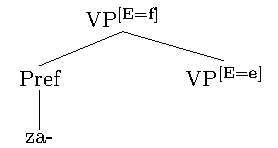
\includegraphics[scale=1]{ZaV.pdf}\\
\begin{forest}
[VP\textsuperscript{[E=\textbf{f}]}
  [Pref [\Prefix{za-}]]
  [VP\textsuperscript{[E=\textbf{e}]}]
]
\end{forest}
\begin{tabular}[t]{ll}
\begin{tabular}[t]{l}
\avm{
\btag{f} [\type*{transition}
      \POST & [\type*{event}
         \MDIM & [\type*{proper-scale}
            \MIN & deg ] 
     ]
   ]
}\\
\end{tabular}
\begin{footnotesize}
\begin{tabular}[t]{@{}l@{}}
$\tuple{\btag{f}\BC\POST,\btag{e}}\D\type{esegm-of}$\\[1ex]
$\tuple{\btag{f}\BC\POST\C\MDIM,\btag{e}\BC\MDIM}\D\type{segm-of}$\\
\end{tabular}
\end{footnotesize}
\\\\
\begin{tabular}[t]{l}
\avm{
\btag{e} [\type*{event}
	 \VERBDIM & \1\\
     \MDIM & \1 [\type*{proper-scale}]
   ]
}
\hfill
\end{tabular}
\end{tabular}
\hfill
\caption{Representation of the contribution of the prefix \Prefix{za-}}
\label{fig.za.frame.semantics}
\end{figure}

The basic frame that I propose in order to represent the general semantic contribution of the prefix \Prefix{za-} is provided on \figref{fig.za.frame.semantics} together with a tree fragment that represents the attachment of the prefix (and belongs to the \isi{metagrammar} description). Informally it can be read in the following way: suppose the \isi{derivational base} denotes some event \textbf{e} that has as its \isi{measure dimension} some scale of type \textit{proper-scale}. Then the verb prefixed with the prefix \Prefix{za-} denotes another event that is of type \textit{transition}. A transition is in general characterised by its anterior and posterior states. In this case we are interested in the posterior state that has to be a segment of the event denoted by the derivation base. What we also know is that the scale in the \isi{measure dimension} of the posterior state of the transition event corresponds to some initial segment of the scale in the \isi{measure dimension} of the event denoted by the \isi{derivational base}. The identity of two attributes {\scshape\VERBDIM} and {\scshape\MDIM} of the event frame on \figref{fig.za.frame.semantics} ensures that the \isi{measure dimension} of the event is determined by the verb.

Let me now illustrate what happens when this prefix is attached to a verb. Consider an indeterminate \isi{motion verb} \textit{begat'} `to run'. The \isi{frame representation} of this verb is provided on the left side of \figref{frame:begat}. It refers to an event of type \textit{translocation} with the manner of motion of type \textit{run}. The motion leaves some trace and it is performed by some actor. Note that there is no \PATH attribute. This is the assumption made and advocated in \citealt{ZinovaOsswald:paper}, as the \TRACE is regarded to be a set of points the object moved through and thus it is present in the description of any event of type \textit{translocation}. The \PATH attribute is taken to have a more complex structure and be present only in case of a directed motion event.

\begin{figure}
\begin{tabular}[t]{l}
\textit{Verbal base in the dictionary}\\
\avm{
\btag{g} [\type*{transloc}
	   \MANN & [\type*{run}]\relax\\
       \ACTOR & \1\\
	   \TRACE & \2
]
}
\end{tabular}
\hfill
\begin{tabular}[t]{c}
\textit{Verb after dimension constructor}\\
\avm{
\btag{g}  [\type*{transloc $\und$ scale $\und$ time}
	   \MANN & [\type*{run}]\relax\\
       \ACTOR & \1\\
	   \TRACE & \2\\
	   \VERBDIM & \btag{g}  
]
}
\end{tabular}
\caption{Frame representation of an indeterminate motion verb \textit{begat'} `to run' \label{frame:begat}}
\end{figure}

The frame on the right side of \figref{frame:begat} is an enriched variant of the frame on the left: here, information about the \isi{verbal dimension} is added. Let me explain the idea behind this enrichment in a bit more detail. I claim that from the point of view of the dimension interpretations, all verbs can be divided in two categories: verbs that have a scale they are related to, and verbs that are more flexible in this respect. In the first category fall such verbs as \textit{stoit'} `to cost' (price scale), \textit{gret'} `to warm up' (temperature scale), \textit{mo\v{c}it'} `to make wet' (degree of \isi{wetness scale}), \textit{letet'} `to fly (directional)' (\isi{path scale}). 

%For those verbs the \isi{measure dimension} is already determined in the basic verb representation and cannot be changed. If the direct object is present, it must be able to provide the same \isi{measure dimension} as is preselected by the verb, usually through the relevant attribute, such as price. Note that such attribute is not necessarily present in the default representation of the object, but can be added, if needed. One can hypothesise that in case the attribute is present by default (e.g., for a house) it would be easier (faster) to use it as a direct object of the verb \textit{stoit'} `to cost' then if such attribute is absent (e.g., for a sky).

The second group of verbs is such that no specific scale is provided in their representation. This means that most of the time these verbs will ``accept'' the \isi{scales} ``offered'' by the direct objects, except for the cases when the prefix demands that the \isi{measure dimension} is determined by the verb. In these situations the representation of the verb has to be enriched with the information about the scale. The only scale that seems to be generally available as the \isi{verbal dimension} is the event itself. So the frame on the right side of \figref{frame:begat} obtains an attribute {\scshape\VERBDIM} with a value of type \textit{scale} that has to be identified with the event itself. The type \textit{scale} then gets conjoined with the type \textit{event}. The separation of the dimension information (if this information is not verb-specific) from the rest of the verbal frame (as it is shown by the different states of the frames on the left and right sights of \figref{frame:begat}) allows for a more compact lexicon representation. At the same time it is also possible to store the enriched representation as a dictionary entry and this is in fact what I have to do in the implementation (see Chapter~\ref{Chapter8}) due to the current restrictions of the formalism. 
 
%This procedure is similar for the verbs and the nouns and could be optimized if the formalism would allow to define a set as a value of an attribute and use any member of the set as a \isi{measure dimension} as long as it satisfies other conditions imposed by the prefix or the \isi{context}. Such solution is sketched in \citealt{Zinova:14}, but as it cannot be implemented in the current framework, I now offer a less elegant, but implementable variant. 

%To enrich verbal representations with verbal measure dimensions in those cases when this dimension is not fixed, I propose to provide a bunch of constructors that can be applied to the verb and output a minimal VP. First such constructor should only accept those verbs that have a predefined \isi{verbal dimension} and change nothing. Next option is to use time dimension, that is generally available for any verb (of course when the \isi{verbal dimension} is already specified, a conflict between the two \isi{scales} will arise, so there is no need to limit such constructor in any respect). As one can see on the middle frame on \figref{frame:begat}, \isi{time scale} is not overtly present: it is realised as coreference of the scale and the event itself. 

%Other constructors that are available for a given verb depend on the attributes is has. For example, the verb \textit{begat'} `to run' can acquire \isi{verbal dimension} of the type \textit{path}, as it has a trace attribute (see the rightmost frame on \figref{frame:begat}). This allows us to explain why in some situations it can be used interchangeably with the directed \isi{motion verb} \textit{be\v{z}at'} `to run', whereas remaining dispreferred. The preference should be then explained in pragmatic terms, as the determinate \isi{motion verb} is more specific and thus should be preferred in all the situations where it is suitable to use the \isi{path scale}.

Now we are ready to unify the verbal frame (on the right side of \figref{frame:begat}) with the prefix frame shown on \figref{fig.za.frame.semantics}. As a result, we obtain the frame for the verb \textit{zabegat'} `to start running' that is presented on \figref{frame:zabegat}. This figure also shows a simplified (no agreement features) \isi{initial tree} for the derived verb.

\begin{figure}
\centering
% % 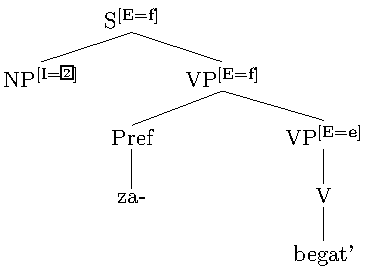
\includegraphics[scale=1]{ZaBegat.pdf}\\
\begin{forest}
[S\textsuperscript{[E=\textbf{f}]}
  [NP\textsuperscript{$\left[\text{I=\avm{\2}}\right]$}]
  [VP\textsuperscript{E=\textbf{f}}
    [Pref [\Prefix{za-}]]
    [VP\textsuperscript{[E=\textbf{e}]} [V [begat']]]
  ]
]
\end{forest}
\begin{tabular}[t]{ll}
\begin{tabular}[t]{l}
\avm{
\btag{f} [\type*{transition}
      \POST & [\type*{event}
         \MDIM & [\type*{proper-scale}
         	\MIN & deg ]
     ]
   ]
}\\
\end{tabular}
\begin{footnotesize}
\begin{tabular}{l}
~\\
~\\
$\tuple{\btag{f}\BC\POST,\btag{e}}\D\type{esegm-of}$\\
$\tuple{\btag{f}\BC\POST\C\MDIM,\btag{e}\BC\MDIM}\D\type{segm-of}$\\
\end{tabular}
\end{footnotesize}
\\\\
\begin{tabular}[t]{l}
\avm{
\btag{e} [\type*{event $\und$ transloc $\und$ proper-scale}
      \MDIM & \btag{e}\\
	   \MANN & [\type*{run}]\\
       \ACTOR & \1\\
	   \TRACE & \2\\
	   \VERBDIM & \btag{e}
]
}\\
\end{tabular}
\end{tabular}
\hfill
\caption{Frame representation of the verb \textit{zabegat'} `to start running'}
\label{frame:zabegat}
\end{figure}

The frame on \figref{frame:zabegat} can be read as follows: the verb \textit{zabegat'} `to start running' denotes an event of type \textit{transition} such that the posterior state is a part of a running event and the minimum degree on the event scale after the transition corresponds to the beginning of running. In other words, the combination of the two frames describes a transition from not running into running, which corresponds to the \isi{inchoative} interpretation. The noun dimension has to agree with the \isi{measure dimension}, which becomes relevant in case a direct object is present.

Now I would like to spell out two processes: the process of selection of a subpart of the scale that is used as a \isi{measure dimension} of the new event and the process of obtaining the minimum degree on this scale. The first step is to recall that self-scaling means to consider the event as being itself a scale. From this we can derive a general rule that the minimum of the event scale is always the start of the event and the maximum of the event scale is always the end of the event, so those attribute-value pairs get equated. As a consequence, for this type of the scale the interpretation of the \Prefix{za-}prefixed verb is \isi{inchoative}, as the posterior state is associated with the initial portion of the event.

I would like to pay attention to one more detail of the analysis: the type of the scale that is used as a \isi{measure dimension}. As defined by the prefix frame, this scale has to be a \textit{proper} scale. As I have proposed in Chapter~\ref{Chapter5}, proper \isi{scales} carry more information than measure of change \isi{scales} and those two types are incompatible (as stated in the \isi{type hierarchy} and repeated as a constraint in \ref{const:proper}). With this assumption we can show why sentences as \ref{ex:zabegat:time} are not acceptable, but first we need to construct the frame for the \isi{time measure expression} \textit{2 \v{c}asa} `for two hours'. 

\ex.\label{const:proper}\textit{proper-scale} $\und$ \textit{measure-of-change} $\rightarrow \bot$

\exg.\label{ex:zabegat:time}\#Vasja zabegal$_{\INDET}$ dva \v{c}asa.\\
Vasya \glb{za}.run.\glb{pst}.\glb{sg}.\glb{m} two hours\\

Let me note that Russian and English time measure expressions are not parallel. For example, the \isi{accusative time measure phrase} \textit{dva \v{c}asa} `for two hours' can become a part of a prepositional construction \textit{za dva \v{c}asa} `in two hours', which is not possible for English \textit{(*in for two hours)}. Furthermore, it can be used in the \textit{v-}headed prepositional phrase to refer to a point in time (\textit{v dva \v{c}asa} `at two o'clock'). Keeping this in mind, I propose to represent the semantics of the measure expression \textit{dva \v{c}asa} `two hours' as shown on the left side of \figref{frame:2hours}. 

\begin{figure}
\begin{tabular}[b]{c}
% % 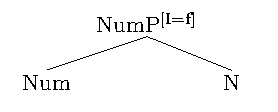
\includegraphics[scale=1]{NumP.pdf}\\
\begin{forest}
[NumP\textsuperscript{[I=\textbf{f}]}
[Num] [N]
]
\end{forest}\\
\avm{
\btag{f} [\type*{length}
  		\VAL & 2\\
  		\MUNIT & hour  
  ]
}
\end{tabular}\hspace{2cm}
\begin{tabular}[b]{c}
% % 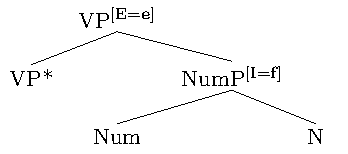
\includegraphics[scale=1]{VNumP.pdf}\\
\begin{forest}
[VP\textsuperscript{[E=\textbf{e}]}
  [VP*]
  [NumP\textsuperscript{[I=\textbf{f}]}
    [Num] [N]
  ]
]
\end{forest}\\
\avm{
\btag{e}[\type*{event}
  \DURATION & \btag{f}[\type*{length}
  		\VAL & 2\\
  		\MUNIT & hour  
  ]
]
}
\end{tabular}
\caption{Frame representation of the time adverbial \textit{dva \v{c}asa} `for two hours' \label{frame:2hours}}
\end{figure}

Such a representation is neutral with respect to further insertion in various types of constructions and is also shared with other measure-related expressions, such as \textit{p'at' kilometrov} `five kilometres' and \textit{tri kilogramma} `three kilograms'.

In order to combine the measure phrase with a verbal phrase, we need to embed it into the verbal construction as shown on the right side of \figref{frame:2hours}. When this is performed, a VP node becomes the head of the phrase, so the measure expression looses the ability to become a part of a prepositional phrase. At the same time another VP node marked as a footnode is created, so now the measure phrase can be adjoined at a VP node.  On the semantic side a new base node of type \textit{event} is created and the initial representation of the measure phrase becomes the value of the \DURATION attribute of this event.

When the verbal phrase is constructed, constraint \ref{constr:duration} is applied. It states that if the type of the frame is \textit{bounded-event}, than the \isi{measure dimension} of this event is of type \textit{measure-of-change} and \textit{time}, the minimum on the scale is \textit{zero} and the maximum is equal to the value of the \isi{duration}.

\ex.\label{constr:duration}\textit{bounded-event} $\und$ (\DURATION = $\top$) $\rightarrow$ ({\scshape\MDIM} = \textit{measure-of-change} $\und$ time) $\und$  {\scshape\MDIM} . \MIN = 0 $\und$ {\scshape\MDIM} . \MAX $\triangleq$ \DURATION .\VAL

%Note that this solution can be improved by creating a system of rules that will assign thematic roles and also determine the slots various measure and path expressions should occupy in the verbal structure. At the moment the asymmetry is explained by the presence of case system that help to determine thematic roles using syntactic information, whereas in the domain of measure expressions only semantic information is left. This problem, however, can be solved, as one can conclude looking at the recent systems of thematic role assignment, such as CITE LAURA?

% the enrichment mechanism is shared with noun phrases in direct object position: for the nouns, their characteristics are stored in the dictionary, but converted to the \isi{measure dimension} only when they appear in certain constructions. 

\begin{figure}
\hfill
\begin{tabular}[t]{@{}cl@{}}
\txt{za}-V &
\begin{tabular}[t]{@{}l@{}}
\avm{
\btag{f} [\type*{transition}
      \POST & \2 [\type*{event}
         \MDIM & \2 [\type*{proper-scale}
            \MIN & deg ] \\
     ]
   ]
}\\
\end{tabular}
\begin{footnotesize}
\begin{tabular}[t]{@{}l@{}}
$\tuple{\btag{f}\BC\POST,\btag{e}}\D\type{esegm-of}$\\[1ex]
$\tuple{\btag{f}\BC\POST\C\MDIM,\btag{e}\BC\MDIM}\D\type{segm-of}$\\
\end{tabular}
\end{footnotesize}
\\\\
V &
\begin{tabular}[t]{@{}l@{}}
\avm{
\btag{e} [\type*{transloc}
	   \DURATION & [\type*{length}
  			\VAL & 2\\
  			\MUNIT & hour  
   		]\\      
      	\MDIM & \btag{e} [\type*{\color{red}\underline{measure-of-change $\und$ proper-scale $\und$ time}}
			\MIN & 0\\      		
     		\MAX & 2
      	]  \\
	   	\MANN & run\\
       \ACTOR & entity\\
	   \TRACE & trace\\
	   \VERBDIM & \btag{e}
]
}\\
\end{tabular}
\end{tabular}
\hfill
\caption{Failure of unification of the frames for \textit{zabegat'} `to start running' and \textit{dva \v{c}asa}  + `for two hours'}
\label{frame:zabegat:2hours}
\end{figure}

Now we can combine the representation on the right side of \figref{frame:2hours} with the representation of the verb \textit{zabegat'} `to start running' provided on \figref{frame:zabegat}. The \isi{unification} in this case leads to a conflict due to the type constraint shown in \ref{const:proper}. The combination of the two frames with the underlined conflict is shown on \figref{frame:zabegat:2hours}. 

To complete the picture, let me show that there is no \isi{unification failure} when the same time measure phrase is combined with a \isi{non-prefixed} verb. In this case the resulting phrase \textit{begat' dva \v{c}asa} `run for two hours' is perfectly acceptable. Indeed, as the \isi{verbal dimension} is required to unify with the \isi{measure dimension} only at the moment of \Prefix{za-}\isi{prefixation}, no conflict arises in this case, as the values of the attributes {\scshape\MDIM} and {\scshape\VERBDIM} remain unrelated. The frame can be read as follows: ``There is an event of \isi{translocation} with manner \textit{run} that some actor is involved in. This \isi{translocation} leaves some trace and has a \isi{duration} of two hours.'' The rest of the frame is not relevant for its final interpretation and, in fact, could be generated at the moment of prefix attachment (this is, however, not possible to implement in the framework I use due to current restrictions of the compiler).

\begin{figure}
\centering
\avm{
\btag{e} [\type*{transloc}
	   \MANN & run\\
       \ACTOR & entity\\
	   \TRACE & trace\\
	   \DURATION & [\type*{length $\und$ time}
  			\VAL & 2\\
  			\MUNIT & hour  
   		]\\ 
	  	\MDIM & [\type*{measure-of-change $\und$ time}
			\MIN & 0\\      		
     		\MAX & 2
   		]\\	   
	   \VERBDIM & \btag{e}
]
}\\fv
\caption{Frame representation of the verbal phrase \textit{begat' dva \v{c}asa} `run for two hours' \label{frame:begat:2hours}}
\end{figure}

As there is nothing special with the indeterminate motion verbs that could influence the process of combining them with the prefix \Prefix{za-}, other verbs that have self-reference (\textit{event} $\wedge$ \textit{scale} type) as the \isi{verbal dimension} acquire \isi{inchoative} interpretation in combination with the prefix \Prefix{za-} in exactly the same way. Let me illustrate this and also the fact that the proposed analysis can be extended to other usages of the prefix \Prefix{za-} (that occur in presence of other \isi{scales}) using as an example the verb \textit{\v{z}eltet'} `to be yellow and be seen/to become yellow' that we have discussed in Chapter~\ref{Chapter5}. First let us construct two frames that reflect two interpretations of the basic imperfective verb that probably follow two semantic schemes associated with deriving verbs from colour terms. Under the first interpretation, the verb refers to a state of the theme. The colour of the theme is (constantly) yellow and the state can be specified as \textit{be seen}. As for any other stative verb, the only available \isi{verbal dimension} is the event (state) itself. 

\begin{figure}\small
\begin{tabular}[t]{@{}c@{}}
\textit{to be yellow and be seen}\\
\avm{
 \btag{e} [\type*{state}
  		\STATE & [\type*{be\_seen}]\\
  		\THEME & \1 [
  			\COLOR & [\type*{yellow}]\relax\\
  		]\\
  		\VERBDIM & \btag{e}
  ]
}
\end{tabular}\hfill\begin{tabular}[t]{@{}c@{}}
\textit{to become yellow}\\
\avm{
\btag{e} [\type*{change-of-state}
  \VERBDIM & \2 [\type*{\isi{property-scale} $\und$ yellow} 
  	\MIN & \3\\
  	\MAX & \4  
  ]\\
  \MDIM & \2\\
  \THEME & \1
]
}
\end{tabular}
\caption{Frame representations of the verb \textit{\v{z}eltet'} `to be yellow and be seen/to become yellow' \label{frame:zeltet}}
\end{figure}

The second interpretation is related to a different kind of event -- a change of state. What we know in this situation is that there is a theme that undergoes a change of state along the property scale, more specifically -- a scale of type \textit{yellow}. Note that representing verbal semantics in detail is not the primary focus of this thesis and verbal frames provided here should probably be revised (especially with respect to an accurate representation of change of colour), but suffice to show how the prefix \Prefix{za-} functions.

Let us unify the frame for the prefix \Prefix{za-} with the frame representations of the verb. We will start with the interpretation of the \isi{derivational base} that makes use of the event scale (`to be yellow and become seen'). Here everything proceeds exactly as in case of the verb \textit{begat'} `to run' and the frame obtained as a result of the \isi{unification} describes an event of type \textit{transition} such that the posterior state of this transition corresponds to the initial stage of the event `be yellow and be seen', where `be yellow' is a constant property of the theme, so this means that the derived verb refers to a beginning of the `be seen' state.

\begin{figure}
\begin{minipage}[b]{.5\textwidth}\centering
\textit{\Prefix{za-} (to be yellow and be seen)}\\
\avm{
\btag{f} [\type*{transition}
      \POST & [\type*{event}
         \MDIM & [\type*{proper-scale}
            \MIN & deg ]
     ]
   ]
}
\end{minipage}%
\begin{minipage}[b]{.5\textwidth}\centering
\avm{
\btag{e}[\type*{state $\und$ proper-scale}
  		\STATE & [\type*{be\_seen}]\\
  		\THEME & \2 [
  			\COLOR & [\type*{yellow}]\relax\\
  		]\\
  		\VERBDIM & \btag{e}\\
  		\MDIM & \btag{e}
  ]
}
\end{minipage}\medskip\\
\begin{tabular}[t]{l}
$\tuple{\btag{f}\BC\POST,\btag{e}}\D\type{esegm-of}$\\[1ex]
$\tuple{\btag{f}\BC\POST\C\MDIM,\btag{e}\BC\MDIM}\D\type{segm-of}$\\
\end{tabular}
\caption{Frame representation of the verb \textit{za\v{z}eltet'} `to be yellow and become seen' \label{frame:zazeltet:seen}}
\end{figure}

Next I would like to show what happens in the other case: when the \isi{verbal dimension} is the colour property scale. Under this interpretation of the \isi{derivational base} the transition should have as its posterior state some part of the original event. Which part the posterior state corresponds to is determined by the \isi{measure dimension} of the derived transition event: the minimum point of the scale has to be included. It is, however, not clear, what the minimum point is, as for the verb \textit{\v{z}eltet'} `to become yellow' it is only given in form of a variable. This means that for the new event (transition) the minimum point on the property scale remains a variable. As a result, we obtain a frame that describes an event of type \textit{transition} with a posterior state corresponding to some yellow state (but we do not know its exact characteristics) of the theme. The \isi{underspecification of the scale} allows for two interpretations of the derived verb in this case: in the minimum on the scale is some point that can be not considered as being yellow, than the derived verb is interpreted as `to start becoming yellow'; if the minimum on the scale is some point that is yellow, then the derived verb is interpreted as `to become yellow'.

In sum, two representations of the verb combined with one prefix representation yield three possible interpretations of the derived verb: `to be yellow and be seen', `to become yellow', and `to start becoming yellow'. This result agrees with the dictionary data that points exactly to these three meanings of the verb \textit{za\v{z}eltet'}. 

\begin{figure}
\textit{za(to become yellow)}\\
\raggedright
\avm{
\btag{e} [\type*{transition}
      \POST & [\type*{event}
         \MDIM & [\type*{\isi{property-scale} $\und$ proper-scale $\und$ yellow}
            \MIN & \3
          ] \\
     ]
   ]
}\medskip\\
\avm{
\btag{f} [\type*{change-of-state}
  \VERBDIM & \2 [\type*{\isi{property-scale} $\und$ proper-scale $\und$ yellow} 
  	\MIN & \3\\
  	\MAX & \4  
  ]\\
  \MDIM & \2\\
  \THEME & \1
]
}\medskip\\\centering
\begin{tabular}[t]{l}
$\tuple{\btag{f}\BC\POST,\btag{e}}\D\type{esegm-of}$\\[1ex]
$\tuple{\btag{f}\BC\POST\C\MDIM,\btag{e}\BC\MDIM}\D\type{segm-of}$\\
\end{tabular}
\caption{Frame representation of the verb \textit{za\v{z}eltet'} `to become yellow/to start becoming yellow' \label{frame:zazeltet:yellow}}
\end{figure}

Another important scale type that can be provided by the verb is \textit{path}. This is the case of determinate motion verbs, such as \textit{be\v{z}at'} `to run (one direction)'. When the \isi{frame representation} of the prefix \Prefix{za-} proposed above is combined with the \isi{frame representation} of such a verb, the resulting interpretation of the derived verb is `transition such that the posterior state is associated with the \isi{locomotion} that starts at the border of the contextually specified region'. This case is analyzed in detail in \citet{ZinovaOsswald:paper}, so I will skip further details here.

As for the \isi{resultative} interpretation, some more details and ideas are provided in \citealt{ZinovaKallmeyer:12} and \citealt{Zinova:14}, which address the locative alternation phenomena that in Russian is related to the \isi{resultative} usage of the prefix \Prefix{za-}. 

\section{Frame semantics for the prefix \textit{na-}}\label{section:frame:na}
The second prefix that we have discussed in Chapter~\ref{Chapter5} is the prefix \Prefix{na-} with its \isi{cumulative} interpretation. As I have concluded after analysing the proposals of \citet{Filip:00} and \citet{Kagan:book} and providing further examples and observations (see discussion in Section~\ref{subsection:semantics:na}), the prefix requires a scale that is provided by the verb and is at the same time a parameter of the object. For example, temperature is a variable parameter for most of the objects, although it may be easier accessible for objects like \textit{soup} than for objects like \textit{book}.


\begin{figure}
\begin{minipage}{0.5\textwidth}
\avm{
\btag{e} [\type*{bounded-event}
	   \NOUNDIM & \3\\       
	   \VERBDIM & \3\\
       \MDIM & \3[\type*{scale}
			\MIN & \1 \\	  
			\THRESHOLD & \2
       ] \\
       \INIT & [\type*{stage}
     		\POS & \1]\\
      \FIN & [\type*{stage} 
  		 	\POS & \4 ]\\
   ]
}\\
\centering
\svar{2} $\leq$ \svar{4}
\end{minipage}\hspace{2cm}\begin{minipage}{0.25\textwidth}
% % 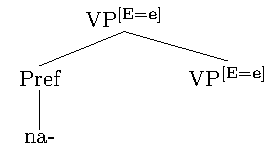
\includegraphics[scale=1]{NaVerb.pdf}\\
\begin{forest}
[VP\textsuperscript{[E=\textbf{e}]}
  [Pref [\Prefix{na-}]]
  [VP\textsuperscript{[E=\textbf{e}]}]
]
\end{forest}
\end{minipage}
\caption{Representation of the contribution of the prefix \Prefix{na-}\label{frame:na}}
\end{figure}

When these requirements are met and the prefix is attached, it maps the minimum point of the scale onto the initial stage of the event and some point that is located at or above the threshold value onto the final stage of the event.  As I have shown earlier, there are cases when a \Prefix{na-}prefixed verb is compatible with a singular object description. Taking this possibility into account, I propose a \isi{frame representation} for the prefix as shown on \figref{frame:na}. This frame encodes the following information: the event denoted by a \Prefix{na-}prefixed verb is a bounded event, the \isi{measure dimension} is at the same time the \isi{verbal dimension} and the noun dimension, the initial stage of the event corresponds to the minimum point of the \isi{measure dimension} scale (that normally is provided by the noun and is identical to the initial value of the relevant property) and the final stage of the event corresponds to the point on the scale that is located at or above the threshold value. 

Note that there is no direct requirement for an \isi{open scale}, but in many cases it automatically emerges from the \isi{semantic restrictions} and pragmatic principles alone. The argumentation proceeds in two steps. First, the semantic representation of the event carries a requirement that the event must continue at least until the threshold value on the relevant scale is reached. At the same time the event cannot continue beyond the maximum value on the scale. This means that if there is a maximum value of the property that is supplied by the noun and no information that this maximum value is at least the threshold value, uttering such verb would be pragmatically unsuccessful. Second, suppose the threshold value equals the maximum value on the scale. Then the final stage of the event has to be related to the scale maximum. This is, however, only a special case of the interpretation of a \Prefix{na-}prefixed verb. If there is another verb that semantically states the equation between the \isi{maximum point} of the scale and the final stage of the event explicitly, it is preferred over the \Prefix{na-}prefixed verb for pragmatic reasons (see Chapter~\ref{Chapter6} for more details). 

For example, the verbal phrase \textit{navarila supa} `she made a lot of soup' is interpreted as the quantity of the soup should be significant. This can be explained in terms of a competition with an alternative description \textit{svarila soup} `she made a soup'. If such alternative is absent, then no pragmatic conflict arises in case the maximum of the scale coincides with the threshold: the verbal phrase \textit{naguglit' film} `to google the film' uses the binary scale of the non-found or found state of the object and the maximum on this scale trivially corresponds to the threshold. As there is no other verb that would explicitly equate the maximum value on the scale with the final state, the phrase \textit{naguglit' film} `to google the film' sounds natural. Note, however, that a change of case of the object (\textit{naguglit' filmov} `to google some films') leads to a change of the \isi{measure dimension} to that of \textit{quantity} that has no inherit maximum and the resulting interpretation is `to find a number of films that is at or above the contextually specified threshold'.

A similar mechanism applies in case another prefixed verb with an \isi{excessive} interpretation is available. Consider the verb \textit{gret'} `to heat' that has derivatives \textit{peregret'} `to overheat' and \textit{nagret'} `to warm up' that both refer to the same \isi{measure dimension}: temperature. The \Prefix{pere-}prefixed verb denotes events the final stage of which is associated with a value strictly above the threshold. In this case the range of events the \Prefix{na-}prefixed verb denotes gets limited to the events the final stage of which is associated with the threshold value (in our example it is heating the object up to the appropriate temperature). When an alternative \Prefix{pere-}prefixed verbs is absent (this, for example, is always the case when the \isi{measure dimension} is of type \textit{quantity}, as in this case the \isi{excessive} interpretation of the prefix \Prefix{pere-} is not possible), the \Prefix{na-}prefixed verb would cover the \isi{excessive} interpretation domain. 

\begin{figure}
\centering
\avm{
\btag{e} [\type*{change-of-state}
	   \MANN & [\type*{heat}]\relax\\
       \ACTOR & \1\\
	   \THEME & \2\\
	   \VERBDIM & \3 [\type*{temperature}]\relax\\
	   \MDIM & \3
]
}
\caption{Frame representation of the verb \textit{gret'} `to heat' \label{frame:heat}}
\end{figure}

With this in mind let us see how the prefix is combined with some verbs that operate on different \isi{scales}. We start with the verb \textit{gret'} `to heat' that has as the \isi{verbal dimension} the temperature scale (that is also copied to the \isi{measure dimension} attribute). When this verb combines with the prefix \Prefix{na-}, the resulting frame (provided on \figref{frame:nagret}) denotes a bounded change of state with manner \textit{heat}, some actor, and some theme that has a temperature attribute. The event starts at the temperature corresponding to the \isi{minimum of the scale} and ends when the temperature is at or above the threshold value. Note that at this moment the minimum on the scale is an unbound variable that will acquire its value later. The threshold value will also be determined only by the pragmatic module that is as well used to block the ``above the threshold'' interpretation of the verb \textit{nagret'} `to warm up', as sketched above.

\begin{figure}
\begin{minipage}{0.6\textwidth}\centering
\avm{
\btag{e} [\type*{\isi{bounded-event} $\und$ change-of-state}
		\MANN & [\type*{heat}]\\
       \ACTOR & \1\\
	   \THEME & \2\\	   
	   \NOUNDIM & \3\\       
	   \VERBDIM & \3\\
       \MDIM & \3[\type*{scale $\und$ temperature}
			\MIN & \4 \\	  
			\THRESHOLD & \5
       ] \\
       \INIT & [\type*{stage}
     		\POS & \4]\\
      \FIN & [\type*{stage} 
  		 	\POS & \6 ]\\
   ]
}\\
\centering
\svar{5} $\leq$ \svar{6}\\
\end{minipage}%
\begin{minipage}{0.4\textwidth}\centering
% % 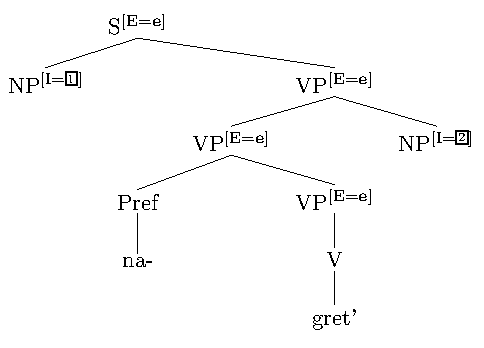
\includegraphics[scale=0.8]{NaGret.pdf}
\begin{forest}
[S\textsuperscript{[E=\textbf{e}]}
  [NP\textsuperscript{[I=\avm{\1}]}]
  [VP\textsuperscript{[E=\textbf{e}]}
   [VP\textsuperscript{[E=\textbf{e}]}
     [Pref [\Prefix{na-}]]
     [VP\textsuperscript{[E=\textbf{e}]} [V [gret']]]
   ]
  [NP\textsuperscript{[I=\avm{\2}]}]
  ]
]
\end{forest}
\end{minipage}
\caption{Representation of the verb \textit{nagret'} `to warm up' \label{frame:nagret}}
\end{figure}

\pagebreak The next step that is relevant for understanding how prefix frames function is the combination of the verb and the direct object. In our case it is a combination of the verb \textit{nagret'} `to warm up' with some appropriate theme, e.g., \textit{sup} `soup'. Here we would need a similar mechanism of enriching noun representations with dimension information, as I have proposed above for the verbs that do not carry \isi{measure dimension} information. In our case (see the frame on \figref{frame:soup:dic}) the object of type \textit{soup} has a temperature attribute, as well as an amount attribute, a kind attribute, and a taste attribute. At the same time \textit{amount} and \textit{temperature} can serve as scalar dimensions, which gives rise to the attributes \AMOUNTDIM and \TEMPDIM.  

\begin{figure}
\centering
\avm{
\btag{f} [\type*{soup}
	   \AMOUNT & [\type*{amount}
	   		\VAL & \1\\
	   		\MUNIT & ml ] \\
       \TEMP & [\type*{temperature}
	   		\VAL & \2\\
	   		\MUNIT & °C ] \\
       \KIND & [\type*{soup-kind}]\\
       \TASTE & [\type*{taste}]\\
       \AMOUNTDIM & [\type*{amount $\und$ measure-of-change}
       		\MIN & 0\\
       		\MAX & \1
       	]\\
       	\TEMPDIM & [\type*{temperature $\und$ proper-scale}
       		\MIN & \2\\ 
       		\MAX & 100
       	]
]
}
\caption{Frame representation of the noun \textit{sup} `soup' \label{frame:soup:dic}}
\end{figure}

Note that the relations between the values of the \AMOUNT and \TEMP attributes of the \textit{soup} and the respective \isi{measure dimension} specifications differ:  in case of the \textit{amount} dimension, the type of the scale is \textit{measure-of-change} and thus the minimum on the scale is 0. The \isi{maximum point} of the scale is the value of the \AMOUNT attribute of the \textit{soup}. In case of the \textit{temperature} dimension the value of the \TEMP attribute serves as a minimum point of the respective dimension. The type of the scale is \textit{proper-scale} and the maximum value is 100 (degrees Celsius).

The \isi{variability of} the minimum or maximum value representation as a static attribute is supported by the variation with respect to which stage is modified by an adjective: if you warm a very cold soup, it is the initial stage of the soup that can be described as \textit{very cold}, but if you write a very long novel, it is the end stage of the novel that can be described as having a length that is greater than the typical length of a long novel. I acknowledge, however, that static representations may prove insufficient: the attribute that provides the relevant dimension undergoes changes and thus is a function of time. However, as such a representation would require significantly more complex modelling and the proposed simplification seems be sufficient for the purposes of current analysis, I will use static representations.

Objects in general may be associated with various measure dimensions, as in case of \textit{soup}, so they have to undergo the process of dimension selection. To perform it, I introduce \textit{dimension constructors} that apply to nouns that have relevant dimensions and identify one of these dimensions with a noun dimension attribute of an event. The first dimension constructor that can be applied to \textit{soup} makes use of the \isi{temperature dimension} of the noun, identifying it with the value of the attribute \NOUNDIM of the event. The event frame gets linked to a VP that linearly precedes the NP (such constructors are part on the \isi{metagrammar} description). The semantic and syntactic parts of the constructor are shown on \figref{constructor:temp}. The result of the \isi{unification} of the \isi{temperature dimension} constructor frame and the \isi{noun phrase} frame is shown on \figref{frame:soup:temp}.

\begin{figure}
\begin{minipage}{0.6\textwidth}
\avm{
\btag{e} [\type*{event}
	\THEME & \btag{f} [\type*{entity}
       	\TEMPDIM & \1
	]\\
	\NOUNDIM & \1
]
}
\end{minipage}
\begin{minipage}{0.35\textwidth}
% % 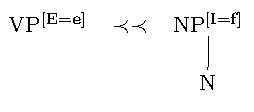
\includegraphics[scale=1]{NaTemp.pdf}
\begin{tikzpicture}[baseline]
\node at (0,0) (VP) {VP\textsuperscript{[E=\textbf{e}]}};
\node (follows) [right = 1em of VP] {$\prec\prec$};
\node [right = 1em of follows] (NP) {NP\textsuperscript{[I=\textbf{f}]}};
\node [below=\baselineskip of NP] (N) {N};
\draw (NP) -- (N);
\end{tikzpicture}
\end{minipage}
\caption{Temperature dimension constructor\label{constructor:temp}}
\end{figure}


\begin{figure}
\centering
\avm{
\btag{e} [\type*{event}
	\THEME & \btag{f} [\type*{soup}
	   \AMOUNT & [\type*{amount}
	   		\VAL & \1\\
	   		\MUNIT & ml ] \\
       \TEMP & [\type*{temperature}
	   		\VAL & \2\\
	   		\MUNIT & °C ] \\
       \KIND & [\type*{soup-kind}]\\
       \TASTE & [\type*{taste}]\\
       \AMOUNTDIM & [\type*{amount $\und$ measure-of-change}
       		\MIN & 0\\
       		\MAX & \1
       	]\\
       	\TEMPDIM & \3 [\type*{temperature $\und$ proper-scale}
       		\MIN & \2\\ 
       		\MAX & 100
       	]
	]\\
	\NOUNDIM & \3
]
}
\caption{Result of unification of the temperature dimension constructor frame with the frame for the noun \textit{sup} `soup'  \label{frame:soup:temp}}
\end{figure}

The second dimension constructor applicable in case of the noun \textit{sup} `soup' is the \isi{amount dimension} constructor. It is similar to the \isi{temperature dimension} constructor shown before, but it also imposes a syntactic requirement for a genitive case of the object. This constructor is shown on \figref{constructor:amount} and the result of the \isi{unification} of its frame part with the representation of the noun \textit{sup} `soup' is provided on \figref{frame:soup:amount}.

\begin{figure}
\begin{minipage}{0.5\textwidth}\centering
\avm{
\btag{e} [\type*{event}
	\THEME & \btag{f} [\type*{entity}
       \AMOUNTDIM & \1
	]\\
\NOUNDIM & \1
]
}
\end{minipage}\begin{minipage}{0.5\textwidth}\centering
% % 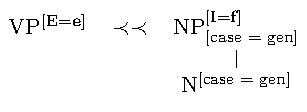
\includegraphics[scale=1]{NPgen.pdf}
\begin{tikzpicture}[baseline]
\node at (0,0) (VP) {VP\textsuperscript{[E=\textbf{e}]}};
\node (follows) [right = 1em of VP] {$\prec\prec$};
\node [right = 1em of follows] (NP) {NP$^{\text{[I=\textbf{f}]}}_{\text{[case = gen]}}$};
\node [below=\baselineskip of NP] (N) {N\textsuperscript{[case = gen]}};
\draw (NP) -- (N);
\end{tikzpicture}
\end{minipage}
\caption{Amount dimension constructor \label{constructor:amount}}
\end{figure}

\begin{figure}
\centering
\avm{
\btag{e} [\type*{event}
	\THEME & \btag{f} [\type*{soup}
	   \AMOUNT & [\type*{amount}
	   		\VAL & \1\\
	   		\MUNIT & ml ] \\
       \TEMP & [\type*{temperature}
	   		\VAL & \2\\
	   		\MUNIT & °C ] \\
       \KIND & [\type*{soup-kind}]\\
       \TASTE & [\type*{taste}]\\
       \AMOUNTDIM & \4 [\type*{amount $\und$ measure-of-change}
       		\MIN & 0\\
       		\MAX & \1
       	]\\
       	\TEMPDIM & [\type*{temperature $\und$ proper-scale}
       		\MIN & \2\\ 
       		\MAX & 100
       	]
	]\\
\NOUNDIM & \4
]
}
\caption{Result of unification of the amount dimension constructor frame with the frame for the noun \textit{sup} `soup' \label{frame:soup:amount}}
\end{figure}

Now we can try combine the representations that emerge from the \isi{unification} of the noun frame with the  frames of \isi{dimension constructors} (\figref{constructor:amount} and \figref{constructor:temp}) with the frame for the verb \textit{nagret'} `to warm up' (\figref{frame:nagret}). First let us use the frame that is produced by the \isi{temperature dimension} constructor (\figref{frame:soup:temp}). The result of inserting the noun representation into the theme slot of the verb in this case is shown on \figref{frame:nagret:soup}. As one can see, now the initial stage of the event corresponds to the initial (minimal) value of the temperature scale associated with the concrete portion of the soup. The final stage is defined as being at least at the threshold value, but not higher than the maximum value. This means that, for example, it would be not possible to heat the soup up to more than 100°C. 

\begin{figure}
\centering
\avm{
\btag{e} [\type*{\isi{bounded-event} $\und$ change-of-state}
		\MANN & [\type*{heat}]\\
       \ACTOR & \3\\
	   \THEME & \btag{f} [\type*{soup}
	   			\AMOUNT & [\type*{amount}
	   			\VAL & \1\\
	   			\MUNIT & ml ] \\
       		\TEMP & [\type*{temperature}
	   			\VAL & \2\\
	   			\MUNIT & °C ] \\
       		\KIND & [\type*{soup-kind}]\\
       		\TASTE & [\type*{taste}]\\
       		\AMOUNTDIM & [\type*{amount $\und$ measure-of-change}
       			\MIN & 0\\
       			\MAX & \1
       		]\\
       		\TEMPDIM & [\type*{temperature $\und$ proper-scale}
       			\MIN & \2\\ 
       			\MAX & 100
      	 	]
		]\\
	   \NOUNDIM & \4\\       
	   \VERBDIM & \4\\
       \MDIM & \4 [\type*{temperature $\und$ proper-scale}
				\MIN & \2\\
       			\THRESHOLD & \5
       ] \\
       \INIT & [\type*{stage}
     		\POS & \2]\\
      \FIN & [\type*{stage} 
  		 	\POS & \6 ]\\
   ]
}\\
\textcolor{white}{dd} \svar{5} $\leq$ \svar{6} $\leq$ \textit{100}
\caption{Frame representation of the verbal phrase \textit{nagret' sup} `to warm up the soup' \label{frame:nagret:soup}}
\end{figure}

What if we try to combine the frame for the verb \textit{nagret'} `to warm up' with the same noun \textit{sup} `soup' that went through another dimension constructor? Let us take the representation shown on \figref{frame:soup:amount} and unify it with the \isi{frame representation} of the verb. When \isi{unification} is performed, it turns out that the \isi{measure dimension} of the event has to be simultaneously of types \textit{temperature} and \textit{amount}. This is not possible due to the constraint \ref{const:temp:amount} on type incompatibility. The type conflict that arises in case the \isi{amount dimension} is selected as the noun dimension is marked on \figref{frame:nagret:soup:amount}. 

\ex.\label{const:temp:amount}\textit{amount} $\und$ \textit{temperature} $\rightarrow \bot$

\begin{figure}
\begin{tabular}{c}
\avm{
\btag{e}  [\type*{\isi{bounded-event} $\und$ change-of-state}
		\MANN & [\type*{heat}]\\
       \ACTOR & \6\\
	   \THEME & \btag{f} [\type*{soup}
	   		\AMOUNT & [\type*{amount}
	   			\VAL & \1\\
	   			\MUNIT & ml ] \\
       		\TEMP & [\type*{temperature}
	   			\VAL & \2\\
	   			\MUNIT & °C ] \\
       		\KIND & [\type*{soup-kind}]\\
       		\TASTE & [\type*{taste}]\\
       		\AMOUNTDIM & \5[\type*{amount $\und$ measure-of-change}
       			\MIN & 0\\
       			\MAX & \1
       		]\\
       		\TEMPDIM & [\type*{temperature $\und$ proper-scale}
       			\MIN & \2\\ 
       			\MAX & 100
      	 	]
		]	\\
	   \NOUNDIM & \5\\       
	   \VERBDIM & \5\\
       \MDIM & \5 [\type*{\textcolor{red}{\underline{temperature $\und$ amount $\und$ measure-of-change}}}
				\MIN & 0\\
       			\THRESHOLD & \3
       ] \\
       \INIT & [\type*{stage}
     		\POS & 0]\\
      \FIN & [\type*{stage} 
  		 	\POS & \4 ]\\
   ]
}\\
\svar{3} $\leq$ \svar{4}
\end{tabular}
\caption{Failure during the unification of the frames for \textit{nagret'} `to warm up and  \textit{sup} `soup' with amount dimension interpretation \label{frame:nagret:soup:amount}}
\end{figure}

The mechanism of type conflict is the main mechanism that prevents un\-want\-ed \isi{prefix stacking} and inappropriate measure phrases or direct object interpretations. Note, however, that noun representations allow for different interpretations and the concrete interpretation is only selected relative to an event. This means that the same noun can be viewed as providing different dimensions when several event nodes are present in the semantic structure. This is even possible with one verb (\isi{secondary imperfective} verb with habitual/\isi{iterative interpretation}) due to different measure dimensions of the iterated subevent and the event that refers to the whole \isi{series of} \isi{subevents}.

Another way of implementing the same system of agreement between the dimensions of the verb and the noun is to formulate requirements (here, for example, a requirement for a temperature scale), but in the current version of the formalisation of Frame Semantics within \isi{XMG} 2 that I am using here it is not possible. For this reason such requirements have to appear implicitly as type or value incompatibilities. I leave it to \isi{future} research to find out whether an approach that uses constructors and type conflicts is cognitively plausible.

%As type constraints are universal (\isi{type hierarchy} is only provided once) and type conflict situations are symmetric. E.g., a type of \textit{open scale} could make sense only for the situations when such scale is inherently open, i.e. no end points might be added by any further specifications; this is so because if one uses this type for any \isi{open scale}, then after the end points are added, the type will become \textit{\isi{open scale} $\und$ close scale}; if these two types are said to be incompatible, we will loose the ability to add end points. If they are compatible, the specification of an \textit{open scale} type is redundant. This symmetry limits the expressive power of the constraint system and I hope that in the near \isi{future} linguists and cognitive scientists will find out which system is cognitively more plausible.

Let me provide one more example of the interaction between the prefix \Prefix{na-}, a verb, and a direct object. This time we will consider the verb \textit{varit'} `to cook' as the base verb. The \isi{frame representation} of this verb is provided on the left side of \figref{frame:varit} and shows that there is no preselected \isi{verbal dimension}. At the same time the frame uncovers the parameter of the cooking event: apart from the type of the theme, the quantity (amount) of the cooked food plays a role. I propose to introduce a dimension constructor that
\begin{enumerate}
\item constructs a \isi{measure dimension} of the type \textit{amount};
\item is only available if the next step is the attachment of the prefix \Prefix{na-};
\item can be applied if the verbal frame contains a specification of the amount of one of the arguments.
\end{enumerate}

If such constructor is used, the verbal representation acquires the corresponding \isi{measure dimension}, as shown on the right side of \figref{frame:varit}. In contrast to the noun \isi{dimension constructors}, no changes on the syntactic side are associated with the \isi{verbal dimension} constructor. At the same time, as stated above, it can be only used in connection with \Prefix{na-}\isi{prefixation}. 

\begin{figure}
\begin{tabular}[t]{l}
\avm{
\btag{e} [\type*{process}
	   \MANN & [\type*{cook}]\relax\\
       \ACTOR & \2\\
	   \THEME & [\type*{food}
	   		\AMOUNT & \1 ]
]
}
\end{tabular}
\hfill
\begin{tabular}[t]{l}
\avm{
\btag{e} [\type*{process}
	   \MANN & [\type*{cook}]\relax\\
       \ACTOR & \2\\
	   \THEME & [\type*{food}
	   		\AMOUNT & \1 ]\\
	   \VERBDIM & [\type*{amount $\und$ measure-of-change}
	   		\MIN & 0\\
	   		\MAX & \1
	   ]
]
}
\end{tabular}
\caption{Frame representation of the verb \textit{varit'} `to cook' before (left) and after (right) an enrichment with scalar information \label{frame:varit}}
\end{figure}

Now the verb has a {\scshape\VERBDIM} argument and can be combined with the prefix frame. The result of the \isi{unification} of the frame on \figref{frame:na} with the frame on the right side of \figref{frame:varit} is shown on \figref{frame:navarit}. It describes a bounded process that starts with no food being cooked and ends when some amount of food that exceeds the threshold is cooked. The \textit{measure-of-change} type of the \textit{amount} scale ensures that there is no requirement for any intermediate event stage to correspond to some intermediate value on the \isi{amount scale}, so no gradual cooking in terms of amount is required, which means that the soup may be prepared as one portion.

\begin{figure}
\begin{tabular}{c}
\avm{
\btag{e}[\type*{\isi{bounded-event} $\und$ process}
		\MANN & [\type{cook}]\relax\\
       \ACTOR & \6\\
	   \THEME & [\type*{food}
	   		\AMOUNT & \1 ]\\
	   \VERBDIM & \2 [\type*{amount $\und$ measure-of-change}
	   		\MIN & 0 \\
	   		\MAX & \1
	   ]\relax\\
	   \NOUNDIM & \2\\   
       \MDIM & \2[\type*{scale}
			\MIN & \3\\	  
			\THRESHOLD & \4\\
       ] \\
       \INIT & [\type*{stage}
     		\POS & 0
      ]\\
      \FIN & [\type*{stage} 
  		 	\POS & \5 
  	]\\
   ]
}\\
\svar{4} $\leq$ \svar{5}\\
\end{tabular}
\caption{Frame representation of the verb \textit{navarit'} `to cook a lot of' \label{frame:navarit}}
\end{figure}

As a next step, we try to combine the representation of the verb \textit{navarit'} `to cook a lot of' with two possible interpretations of the noun \textit{sup} `soup' that we have discussed above (see \figref{frame:soup:temp} and \figref{frame:soup:amount}). Here the result is opposite to that with the verb \textit{nagret'} `to warm up': the temperature-related interpretation of the noun fails to serve as the theme of the event, while the amount interpretation can be successfully used. The \isi{unification failure} in the first case is due to the type conflict that is marked on \figref{frame:navarit:soup:temp}. The type compatibility constraints are violated two times: \textit{amount} conflicts with \textit{temperature} \ref{const:temp:amount} and \textit{proper-scale} conflicts with \textit{measure-of-change} \ref{const:proper}.

\begin{figure}
\begin{tabular}{c}
\avm{
 \btag{e} [\type*{\isi{bounded-event} $\wedge$ process}
		\MANN & [\type*{cook}]\relax\\
       \ACTOR & \1\\
	   \THEME & [\type*{soup}
	   		\AMOUNT & [\type*{amount}
	   			\VAL & \4\\
	   			\MUNIT & ml ] \\
       		\TEMP & \btag{f} [\type*{temperature}
	   			\VAL & 0\\
	   			\MUNIT & °C ] \\
       		\KIND & [\type*{soup-kind}]\\
       		\TASTE & [\type*{taste}]\\
       		\AMOUNTDIM & [\type*{amount $\wedge$ measure-of-change}
       			\MIN & 0\\
       			\MAX & \1
       		]\\
       		\TEMPDIM & \3
		]	\\
	   \NOUNDIM & \3\\       
	   \VERBDIM & \3\\
       \MDIM & \3 [\type*{\textcolor{red}{\underline{amount $\wedge$ temperature  $\wedge$ measure-of-change $\wedge$ proper-scale}}}
				\MIN & 0\\
				\MAX & 100\\       
       			\THRESHOLD & \5
       ] \\
       \INIT & [\type*{stage}
     		\POS & 0 ]\\
      \FIN & [\type*{stage} 
  		 	\POS & \6 ]\\
   ]
}\\
\svar{5} $\leq$ \svar{6} $\leq$ \textit{100}
\end{tabular}
\caption{Failure of unification of the frame for the verb \textit{navarit'} `to cook a lot of' and the frame for the noun \textit{sup} `soup' with temperature dimension interpretation \label{frame:navarit:soup:temp}}
\end{figure}

Note that this representation format stores a lot of world knowledge: not only the resulting verbal frame in case of the verb \textit{nagret'} `to warm up' contains information that the event of warming something proceeds along the temperature scale, but the frame for the verb \textit{navarit'} `to cook' also carries the knowledge that it is not the temperature domain that is relevant in this case, although temperature changes are definitely present during the cooking process. At the same time selection of the \isi{amount dimension} of the verb is a special case and the proposed architecture does not prevent the event from being measured in other terms (e.g., degree of being cooked) when the verb is prefixed with other prefixes.

Now, when we combine the appropriate amount-related representation of the noun \textit{sup} `soup' (in genitive case) with the frame for the verb \textit{navarit'} `to cook a lot of', \isi{unification} is successfully performed. The resulting frame for the verbal phrase \textit{navarit' supa} `to cook a lot of soup', shown on \figref{frame:navarit:soup:amount}, can be read as follows: a bounded process of cooking is performed by some actor. The theme of the event is \textit{soup} that was not present (zero amount value) at the initial stage, but is present at the final stage of the event. The amount of soup cooked at the end of the event equals or exceeds the threshold value. 

\begin{figure}
\begin{tabular}{c}
\avm{
\btag{e} [\type*{\isi{bounded-event} $\und$ process}
		\MANN & [\type*{cook}]\\
       \ACTOR & \2\\
	   \THEME & \btag{f} [\type*{soup}
	   		\AMOUNT & [\type*{amount}
	   			\VAL & \1\\
	   			\MUNIT & ml ] \\
       		\TEMP & [\type*{temperature}
	   			\VAL & 0\\
	   			\MUNIT & °C ] \\
       		\KIND & [\type*{soup-kind}]\\
       		\TASTE & [\type*{taste}]\\
       		\AMOUNTDIM & \3 \\
       		\TEMPDIM & [\type*{temperature $\und$ proper-scale}
       			\MIN & 0\\ 
       			\MAX & 100
      	 	]
		]	\\
	   \NOUNDIM & \3\\       
	   \VERBDIM & \3\\
       \MDIM & \3 [\type*{amount  $\und$ measure-of-change}
				\MIN & 0\\
       			\THRESHOLD & \4\\
       			\MAX & \1
       ] \\
       \INIT & [\type*{stage}
     		\POS & 0 ]\\
      \FIN & [\type*{stage} 
  		 	\POS & \5 ]\\
   ]
}\\
\svar{4} $\leq$ \svar{5} $\leq$ \svar{1}
\end{tabular}
\caption{Frame representation of the verbal phrase \textit{navarit' supa} `to cook a lot of soup' (amount dimension interpretation of the noun) \label{frame:navarit:soup:amount}}
\end{figure}


\section{Frame semantics for the prefix \textit{po-}}\label{section:frame:po}
The next prefix I provide a \isi{frame representation} of is \Prefix{po-}. In Chapter~\ref{Chapter5} on the basis of the analyses proposed by \citet{Filip:00} and \citealt{Kagan:book} and an extensive data discussion, I have concluded that all the usages of the prefix \Prefix{po-} can be unified under one underspecified semantic representation. As has already been observed by \citet{Kagan:book}, the prefix \Prefix{po-} can be attached to different types of \isi{scales}. In the default case, the scale is one of the verbal \isi{scales}. In addition, if the event denoted by the \isi{derivational base} is of type \textit{iteration}, a \textit{cardinality} scale can be provided by the direct object and used as an event scale. As shown on the left side of \figref{frame:po:delim}, the prefix adds information that the event is bounded and the initial and the final stages of the event are related to arbitrary points on the scale.

\begin{figure}
\begin{minipage}{0.4\textwidth}
\avm{
\btag{e} [\type*{bounded-event}
   	   \VERBDIM & \1\\
       \MDIM & \1 [\type*{scale}] \\
       \INIT & [\type*{stage}
     		\POS & \2]\\
       \FIN & [\type*{stage} 
  		 	\POS & \3 ]\\
   ]
}
\end{minipage}
\begin{minipage}{0.55\textwidth}
\avm{
 \btag{e} [\type*{\isi{bounded-event} $\und$ transloc $\und$ scale}
   		\MANN & [\type*{run}]\\
   		\ACTOR & \1\\
   		\TRACE & [\type*{trace}]\\
   	   \VERBDIM &  \btag{e}\\
       \MDIM & \btag{e}\\
       \INIT & [\type*{stage}
     		\POS & \2]\\
       \FIN & [\type*{stage} 
  		 	\POS & \3 ]\\
   ]
}
\end{minipage}
%% Add requirement that if m-dim = path, path-start = init
\caption{Frame representations of the prefix \Prefix{po-} (left) and of the verb \textit{pobegat} `to run for some time' (right) \label{frame:po:delim}}
\end{figure}

Although the prefix does not provide information about the exact scalar degrees associated with the initial and final stages of the event, in some cases the derived verb carries such information. This happens when the \isi{measure dimension} is the event itself and thus the \MIN and \MAX attributes of the scale become promoted to the event level. In this case the initial and the final stages need to be identified with the maximum and the minimum points on the scale. This is done via constraints shown under \ref{rule:minmaxevent}.

\ex.\label{rule:minmaxevent}\a. \MIN = $\top$ $\und$ \INIT = $\top$ $\rightarrow$ \INIT.\POS $\triangleq$ \MIN
\b. \MAX = $\top$ $\und$ \FIN = $\top$ $\rightarrow$ \FIN.\POS $\triangleq$ \MAX

Let us now combine the \isi{frame representation} of the prefix \Prefix{po-} with the verbal frames that we have already considered above. The first verb is an indeterminate \isi{motion verb} \textit{begat'} `to run'. The only dimension constructor the prefix \Prefix{po-} has access to (in case the verb has no specified \isi{measure dimension}) is the self-scaling constructor. This means that the prefix frame can be combined with the frame on the right side of \figref{frame:begat}. The result of the \isi{unification} of the enriched verbal frame with the prefix frame (\figref{frame:po:delim}) is provided on the right side of \figref{frame:po:delim}. The derived frame can be interpreted as describing a bounded event of \isi{translocation} with manner \textit{run}, some actor and some trace, that started at some point and ended at some other point. To ensure that the two degrees on the scale differ from each other, I assume a general constraint shown in \ref{const:diff}.

\ex.\label{const:diff}\textit{bounded-event} $\rightarrow$ \INIT.{\POS} $\neq$ \FIN.\POS

If now this verb is combined with a temporal measure phrase, such as \textit{dva \v{c}asa} `two hours' (see the frame on the right side of \figref{frame:2hours}), the verbal phrase \textit{pobegat' dva \v{c}asa} `to run for two hours' receives the \isi{frame representation} shown on \figref{frame:pobegat:2hours}. Two things has to be taken into account at this point due to the fact that the \isi{measure dimension} is the event itself. First, all the information about the \isi{measure dimension} needs to be ``passed'' to the event level. Afterwards, constraints \ref{constr:duration} and \ref{rule:minmaxevent} are applied. As a result, (1) the event representation acquires the \isi{complex type} \textit{\isi{bounded-event} $\und$ transloc $\und$ scale $\und$ measure-of-change $\und$ time}, (2) the minimum of the \isi{measure dimension} is equated with the minimum of the event and with the scale degree that corresponds to the initial stage of the event, and (3) the maximum of the \isi{measure dimension} is equated with the maximum of the event and with the scale degree that corresponds to the final stage of the event.

\begin{figure}
\centering
\avm{
   \btag{e}[\type*{\isi{bounded-event} $\und$ transloc $\und$ measure-of-change $\und$ time}
   		\MANN & [\type*{run}]\\
   		\ACTOR & [\type*{entity}]\\
   		\TRACE & [\type*{trace}]\\
   		\DUR & [\type*{length $\und$ time}
			\VAL & 2\\
			\MUNIT & hour   		
   		]\\
   	   \VERBDIM &  \btag{e}\\
       \MDIM &  \btag{e}\\
       \INIT & [\type*{stage}
     		\POS & 0]\\
       \FIN & [\type*{stage} 
  		 	\POS & 2]\\
  		\MIN & 0\\
  		\MAX & 2
   ]
}\\
%% Add requirement that if m-dim = path, path-start = init
\caption{Frame semantics of the verbal phrase \textit{pobegat dva \v{c}asa} `to run for two hours' \label{frame:pobegat:2hours}}
\end{figure}


In order to see how the representation of the prefix \Prefix{po-} interacts with other verbal \isi{scales}, let us consider the verb \textit{gret'} `to heat' that denotes a change along the \isi{temperature dimension} (\figref{frame:heat}). The derived verb \textit{pogret'} `to warm up' refers to a bounded change of state of the theme. This change happens along the \isi{temperature dimension}, but no particular values are associated with the initial and the final stages of the event. The resulting frame can be interpreted as `there is an event of manner \textit{heat} that lead to some increase of the temperature'.

\begin{figure}
\centering
\avm{
 \btag{e} [\type*{\isi{bounded-event} $\und$ change-of-state}
   		\MANN & [\type*{heat}]\\
   		\ACTOR & [\type*{entity}]\\
   		\THEME & [\type*{entity}]\\
   	   \VERBDIM & \1 [\type*{temperature}]\\
       \MDIM & \1\\
       \INIT & [\type*{stage}
     		\POS & \2 ]\\
       \FIN & [\type*{stage} 
  		 	\POS & \3 ]
   ]
}\\
%% Add requirement that if m-dim = path, path-start = init
\caption{Frame semantics of the verb \textit{pogret'} `to warm up' \label{frame:pogret}}
\end{figure}

Now let us proceed to the case when the prefix \Prefix{po-} is interpreted distributively. This occurs when an argument of the verb supplies a \isi{cardinality scale} that is used to measure the event. For this situation to be available, the initial event has to be of type \textit{iteration} or has to be compatible with such interpretation.\footnote{In the latter case the \isi{distributive} interpretation usually has to be supported by an overt quantifier.} The only special tool that we need to account for this case is the constraint \ref{const:card} that introduces \textit{iteration} type in case something of type \textit{event} is simultaneously of type \textit{cardinality}. 

\ex.\label{const:card}\textit{event $\und$ cardinality $\rightarrow$ iteration}

%This frame refers to a bounded iteration event that is measured using the \isi{cardinality scale} without strict \isi{internal} structure (this means that several objects may be affected at the same time). The event starts when 0 members of the set the cardinality of which is used as a \isi{measure dimension} are affected and ends when all the members of that set are affected. 
%\begin{figure}
%\centering
%\avm{
%\btag{e}  [\type*{bounded-event}
%   \NOUNDIM & \3\\
%    \MDIM & \3 \[
%       \type*{cardinality}
%       \MIN & \1\\
%       \MAX & \2]\\
%    \INIT & [\type*{stage}
%       \POS & \1 ]\\
%     \FIN & [\type*{stage}
%       \POS & \2 ]
%  ]
%}
%\caption{Semantic representation of a \Prefix{po-}prefixed verb \label{frame:po:distr}}
%\end{figure}
 
 \begin{figure}
% \begin{minipage}{0.45\textwidth}
\hfill\avm{
\btag{e} [\type*{event $\und$iteration}
    \MANN & [\type*{burst}]\\
    \ACTOR & \1\\
    \THEME & \2\\
    \VERBDIM & \btag{e}
  ]
}
% \end{minipage}
% \begin{minipage}{0.5\textwidth}
\hfill%
\avm{
\btag{e} [\type*{iteration $\und$ \isi{bounded-event} $\und$ scale}
    \MANN & [\type*{burst}]\\
    \ACTOR & \1\\
    \THEME & \2\\
    \VERBDIM & \btag{e}\\
    \MDIM & \btag{e} \\
    \INIT & [\type*{stage}
     		\POS & \3]\\
    \FIN & [\type*{stage} 
  		 	\POS & \4 ]\\
  ]
}\hfill%
% \end{minipage}
\caption{Frame representations of the verbs \textit{lopat'} `to burst' (left) and \textit{polopat'} `to burst for some time/all of' (right) \label{frame:lopat}}
\end{figure}
 
Let us consider the case where a non-quantified object can cause the \isi{distributive} interpretation of the verb. To do this, we will look at the semantics of the verb \textit{lopat'} `to burst' and its derivatives. As an event of bursting is punctual, the default interpretation of the imperfective verb is iterative, so the type of the frame on \figref{frame:lopat} is \textit{iteration}. The \isi{verbal dimension} is the event itself. When this verb is prefixed with \Prefix{po-}, the result of the \isi{unification} is the frame shown on the right side of \figref{frame:lopat}.

\begin{figure}
\small
\avm{
\btag{e} [\type*{event}
	\THEME & \btag{f} [\type*{entity}
       \CARD & [\type*{cardinality}
       		\POS & \1
       	]
	]\\
\MDIM & [\type*{cardinality}
			\MIN & 0\\
       		\MAX & \1
       	]
]
}
\hspace{1em}\normalsize%
% % 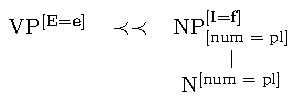
\includegraphics[scale=1]{NPpl.pdf}
\begin{tikzpicture}[baseline]
\node at (0,0) (VP) {VP\textsuperscript{[E=\textbf{e}]}};
\node (follows) [right = 1em of VP] {$\prec\prec$};
\node [right = 1em of follows] (NP) {NP$^{\text{[I=\textbf{f}]}}_{\text{[num = pl]}}$};
\node [below=\baselineskip of NP] (N) {N\textsuperscript{[num = pl]}};
\draw (NP) -- (N);
\end{tikzpicture}
\caption{Cardinality dimension constructor\label{constructor:cardinality}}
\end{figure}

The second ``ingredient'' for the verbal phrase \textit{polopat' \v{s}ary} `to burst the balloons' is the noun \textit{\v{s}ar} `balloon' that has to supply some \isi{measure dimension}, which in this case is the \isi{cardinality scale}. The constructor of the \isi{cardinality scale}, shown on \figref{constructor:cardinality}, is similar to the constructors introduced before. What differs on the syntactic side is the presence of the requirement for the plural number of the noun. As for the semantic side, here the information about the scale of the event is passed directly into the \MDIM attribute and not into the \NOUNDIM attribute. Informally speaking, this means that once the \isi{cardinality constructor} applies, the \isi{cardinality scale} must be used. At the same time the usage of this constructor needs to be restricted to cases when the noun is a direct object of a verb that denotes an event of type \textit{iteration}. 

The \isi{frame representation} of the noun \textit{\v{s}ar} `balloon' is shown on the right side of \figref{frame:balloon}. The right side of the same figure shows the result of \isi{unification} of the noun representation with the cardinality dimension constructor.

\begin{figure}
% \begin{minipage}{0.4\textwidth}
\avm{
\btag{f} [\type*{balloon}
	   \CARD & [\type*{cardinality}
       		\POS & \1
       	]\\
       \SIZE & \2\\
       \COLOR & \3
]
}
% \end{minipage}
\hfill%
% \begin{minipage}{0.575\textwidth}
\avm{
\btag{e} [\type*{event $\und$ iteration}
	\THEME & \btag{f} [\type*{balloon}
	   \CARD & [\type*{cardinality}
       		\POS & \1
       	]\\
       \SIZE & \2\\
       \COLOR & \3]\\
    \MDIM & [ \type*{cardinality}
        \MIN & 0\\
       	\MAX & \1 ]
]
}
% \end{minipage}
\caption{Frame representations of the noun  \textit{\v{s}ar} `balloon' (left) and of the result of its unification with the cardinality dimension constructor (right) \label{frame:balloon}}
\end{figure}

Now we are ready to combine the verbal and the nominal frames and obtain the representation of the verbal phrase \textit{polopat' \v{s}ary} `to burst the balloons' that is shown on \figref{frame:burst:balloon}. The frame describes a bounded iteration event of bursting. The actor is not yet specified, and the theme is of type \textit{balloon} with some cardinality, size, and colour. The event is measured along the cardinality dimension: it starts when zero balloons are burst and ends when all the balloons are burst. There is no information about the \isi{internal} structure of the bursting event, apart from the \textit{iteration} type. This means that several balloons could be burst at once as long as there are multiple bursting sub-events.

\begin{figure}
\centering
\avm{
\btag{e} [\type*{\isi{bounded-event} $\und$ iteration $\und$ cardinality}
    \MANN & [\type*{burst}]\relax\\
    \ACTOR & \5\\
    \THEME & [\type*{balloon}
	   \CARD & [\type*{cardinality}
       		\POS & \1
       	]\\
       \SIZE & \2\\
       \COLOR & \3\\
    ]\\
    \VERBDIM & \btag{e}\\
    \MDIM & \btag{e}\\
    \MIN & 0\\
    \MAX & \1\\
    \INIT & [\type*{stage}
       \POS & 0 ]\\
     \FIN & [\type*{stage}
       \POS & \1 ]
  ]
}\\
\hfill
\caption{Frame representation of the verbal phrase \textit{polopat' \v{s}ary} `to burst the balloons' \label{frame:burst:balloon}}
\end{figure}

Note that the interpretation of the same phrase that describes the bursting event only in terms of time is also possible. As the prefix frame in case of \Prefix{po-} only requires the \isi{verbal dimension} to be present, the application of the dimension constructor is not obligatory. This means that we can unify directly the frame for the verb \textit{polopat'} `to burst for some time/all of' on the right side of \figref{frame:lopat} and the frame for the noun \textit{\v{s}ar} `balloon' provided on the left side of \figref{frame:balloon}. The result of this \isi{unification} is shown on \figref{frame:burst:delim}. Such an interpretation of the verbal phrase \textit{polopat' \v{s}ary} `to burst balloons' is indeed possible and can be paraphrased as `to spend some time bursting balloons'. 

\begin{figure}
\centering
\avm{
\btag{e} [\type*{\isi{bounded-event} $\und$ iteration $\und$ scale}
    \MANN & [\type*{burst}]\relax\\
    \ACTOR & \6\\
    \THEME & [\type*{balloon}
	   \CARD & \1\\
       \SIZE & \2\\
       \COLOR & \3
    ]\\
    \VERBDIM & \btag{e}\\
    \MDIM & \btag{e}\\
    \INIT & [\type*{stage}
       \POS & \4 ]\\
     \FIN & [\type*{stage}
       \POS & \5 ]
  ]
}\\
\hfill
\caption{Frame representation of the verbal phrase \textit{polopat' \v{s}ary} `to burst balloons for some time' \label{frame:burst:delim}}
\end{figure}

\section{Frame semantics for the prefix \textit{pere-}}\label{section:frame:pere}
The next prefix, \Prefix{pere-}, is the most polysemous of Russian verbal prefixes. As I have argued in Section~\ref{subsection:semantics:do}, starting with the proposals of \citet{Demjjanow:97} and \citet{Kagan:book} and providing further data and observations, several representations are required to acquire different interpretations of the prefix, although the process of selection is fully dependent on the type of the scale.

The first representation accounts for \isi{spatial} (crossing), time-related (passing the time, waiting), and \isi{distributive} usages. It applies when the \isi{measure dimension} is such scale that there is a possibility to map each degree on the scale onto the event stages. In particular, this requires the scale to be closed. The second representation applies when there is only one marked point on the relevant scale (e.g., \isi{excessive} and `outdo' usages). In this case the event proceeds from some point below the marked point through the marked point point to the point above it. The last representation leads to the \isi{iterative interpretation} of the event. In this case the derived verb refers to a new event that has as its \isi{preparatory phase} the event denoted by the \isi{derivational base}. I will now show these representations one by one. 

\subsection{Distributive, crossing and waiting interpretations}
The first \isi{frame representation} is, on the one hand, the most `ordinary', as it resembles a lot the frames we have already discussed. On the other hand, it covers three ``traditional'' usages. As we have already discussed a number of similar frames, I will now only point out what is special in this case (the frame is shown on \figref{frame:pere:distr}). As before, the key restrictive factor is the type of the \isi{measure dimension}: a closed \isi{proper scale} in this case. The source of this scale is the noun, if it is not already specified by the verb (in this case the noun has to offer an appropriate scale). The initial and final stages of the event correspond to the minimum and maximum points on the scale. 

\begin{figure}
\centering
\avm{
\btag{e}  [\type*{bounded-event}
   \NOUNDIM & \3\\
    \MDIM & \3 [
       \type*{\isi{closed-scale} $\und$ proper-scale}
       \MIN & \1\\
       \MAX & \2]\\
    \INIT & [\type*{stage}
       \POS & \1 ]\\
     \FIN & [\type*{stage}
       \POS & \2 ]
  ]
}
\caption{Frame representation of the prefix \Prefix{pere-}: case of a closed scale \label{frame:pere:distr}}
\end{figure}

Let me now illustrate how this prefix frame combines with the representations of the verbs. First consider the verb \textit{zimovat'} `to spend winter time' that we have discussed in Chapter~\ref{Chapter6}. This verb has as the \isi{verbal dimension} the \isi{time scale}, as many verbs, but this scale is predefined already in the lexicon, so no choice of \isi{dimension constructors} is possible. The frame for this verb is shown on \figref{frame:zimovat}. (The choice of the type of the manner and the representation of the extremes of the scale may be revised.) Note that the fact that the verbal frame contains information about the minimum and the maximum of the scale does not lead to a bounded interpretation of the verb: it arises only in presence of the \INIT and \FIN attributes.

\begin{figure}
\centering
\avm{
  \btag{e} [\type*{process $\und$ closed-scale}
    \MANN & [\type*{spend-time $\und$ winter}]\\
    \ACTOR & \1\\
    \VERBDIM & \btag{e}\\
    \MDIM & \btag{e}\\
    \MIN &  [\type*{winter-start}]\\
    \MAX &  [\type*{winter-end}]\\
  ]
}\\
\hfill
\caption{Frame representation of the verb \textit{zimovat'} `to spend winter time' \label{frame:zimovat}}
\end{figure}

Now we can combine the frame for the verb \textit{zimovat'} `to spend winter time' with the frame for the prefix \Prefix{pere-}. The result of the \isi{unification} of the two frames is shown on \figref{frame:perezimovat}. This new frame refers to a bounded process of spending winter time that starts when the winter starts and ends when the winter ends. In other words, it is an event of spending the whole winter, which corresponds to the meaning of the verb. The identity of the scale minimum with the initial stage of the event and of the scale maximum with the final stage of the event is established due to the constraints shown in \ref{rule:minmaxevent}.

\begin{figure}
\centering
\avm{
\btag{e} [\type*{process $\und$ \isi{bounded-event} $\und$ \isi{closed-scale} $\und$ proper-scale}
    \MANN & [\type*{spend-time $\und$ winter}]\\
    \ACTOR & \3\\
    \VERBDIM & \btag{e}\\
    \NOUNDIM & \btag{e}\\
    \MDIM & \btag{e}\\
    \MIN &  \1 [\type*{winter-start}]\\
    \MAX &  \2 [\type*{winter-end}]\\
     \INIT & [\type*{stage}
       \POS & \1 ]\\
     \FIN & [\type*{stage}
       \POS & \2 ]
  ]
}
\caption{Frame representation of the verb \textit{perezimovat'} `to spend the winter' \label{frame:perezimovat}}
\end{figure}

The second example is the case of the \isi{path scale}. Consider a determinate \isi{motion verb} \textit{be\v{z}at'} `to run'. The \isi{frame representation} of this verb (on the left side of \figref{frame:bezhat}) differs from the \isi{frame representation} of the indeterminate \isi{motion verb} \textit{begat'} `to run' (shown on \figref{frame:begat}) in that it contains a \PATH attribute and the \textit{path} scale is selected as a \isi{measure dimension}. 

\begin{figure}\small
\avm{
\btag{e} [\type*{transloc}
	   \MANN & [\type*{run}]\\
       \ACTOR & \1\\
	   \TRACE & [\type*{trace}]\\
	   \PATH & \2 [\type*{path}]\\
	   \VERBDIM & \2\\
	   \MDIM & \2
]
}
\hfill
\avm{
\btag{e} [\type*{\isi{bounded-event} $\und$ transloc}
	   	\MANN & [ \type*{run} ]\\
       	\ACTOR & \4\\
	   \PATH & \1\\
	   	\TRACE & [ \type*{trace} ]\\
	   	\VERBDIM & \1 \\
	   	\MDIM & \1 [ \type*{path $\und$ \isi{closed-scale} $\und$ proper-scale}
       		\MIN & \2\\
       		\MAX & \3
       	]\\
      	\NOUNDIM & \1\\
    	\INIT & [\type*{stage}
       		\POS & \2 ]\\
     	\FIN & [\type*{stage}
       		\POS & \3 ]
  ]
}
\caption{Frame representations of the determinate motion verb \textit{be\v{z}at'} `to run' (left) and of the verb \textit{perebe\v{z}at'} `to run accross' (right) \label{frame:bezhat}}
\end{figure}

When the verb \textit{be\v{z}at'} `to run' combines with the prefix \Prefix{pere-}, the frame for the derived verb refers to a bounded \isi{translocation} event of manner \textit{run} that is measured according to the \textit{path} that has to be also the \isi{measure dimension} of the noun. The event starts at the minimum point of the path and ends at the \isi{maximum point} of the path. This frame is shown on the right side of \figref{frame:bezhat}.

What is still missing in this frame is the specification of the path that has to come from the noun. This has to be a closed path across the object the noun refers to. I propose to use a dimension constructor that takes as its input any object that has width or diameter (or, probably, some other attribute) and outputs a path across this object. This path is probably still underspecified, as information from the \isi{context} is needed to find out at least on which ``side'' of the landmark the movement starts. So if we start with a dictionary noun representation, such as shown on the left side of \figref{frame:road}, it can be unified with the constructor shown on \figref{constructor:path}. This constructor is similar to those we have already seen. It specifies the \NOUNDIM attribute of the event as being of type \textit{path}. This path is located in the \LOC of the landmark. The extreme points of this path belong to the set of the edge points of the landmark. There should be an extra condition that ensures that the path goes to the ``opposite'' side, but this is hard (if possible) to formalise (at least in the purely semantic terms and especially for such objects that do not have distinct edges, e.g., a lake), so I will leave this problem for \isi{future} research.  

\begin{figure}\small
\begin{minipage}{0.33\textwidth}\centering
\avm{
\btag{e} [ \type*{event}
	\PATH & \1 [ \type*{path}
		\MIN & \2\\
		\MAX & \3
	]
]
}\end{minipage}\hfill%
\begin{minipage}{0.33\textwidth}\centering
\avm{
\btag{f} [\type*{landmark}
       	\EDGE & \4 \\
       	\LOC & \5 ]
}\\
\svar{1} $\in$ \svar{5} $\und$ \svar{2} $\in$ \svar{4} $\und$ \svar{3} $\in$ \svar{4}
\end{minipage}\hfill%
\begin{minipage}{0.33\textwidth}\centering
% 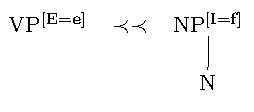
\includegraphics[scale=.8]{NaTemp.pdf}
\begin{tikzpicture}[baseline]
\node at (0,0) (VP) {VP\textsuperscript{[E=\textbf{e}]}};
\node (follows) [right = 1em of VP] {$\prec\prec$};
\node [right = 1em of follows] (NP) {NP\textsuperscript{[I=\textbf{f}]}};
\node [below=\baselineskip of NP] (N) {N};
\draw (NP) -- (N);
\end{tikzpicture}
\end{minipage}
\caption{Path dimension constructor\label{constructor:path}}
\end{figure}

\begin{figure}\small
% \begin{minipage}{0.35\textwidth}
\avm{
\btag{f} [\type*{road}
	   \WIDTH & \1\\
	   \LOC & \2\\
	   \EDGE & \3
]
}\hfill%
% \end{minipage}
% \begin{minipage}{0.25\textwidth}
\avm{
\btag{e} [\type*{event}
	\PATH & \6[\type*{path}
		\MIN & \4\\
		\MAX & \5
	]
]
}\hfill%
% \end{minipage}
\begin{minipage}{0.275\textwidth}
\avm{
\btag{f} [\type*{landmark $\und$ road}
	   \WIDTH & \1\\
	    \LOC & \2\\
       	\EDGE & \3 ]
}\smallskip\\
\svar{4} $\in$ \svar{3} $\und$ \svar{5} $\in$ \svar{3} $\und$ \svar{6} $\in$ \svar{2}
\end{minipage}
\caption{Frame representations of the noun \textit{doroga} `road' (left) and of its unification with the path dimension constructor (right) \label{frame:road}}
\end{figure}

Now we are ready to combine the verbal frame that is shown on the right side of \figref{frame:bezhat} with the noun representation that is unified with the dimension constructor (shown on the right side of \figref{frame:road}. The result of the \isi{unification} is provided on \figref{frame:cross:road}. In the derived frame the noun contributes information about the path across the landmark that becomes the \isi{measure dimension} of the event.

\begin{figure}
\small
\begin{minipage}{0.6\textwidth}
\avm{
\btag{e} [\type*{\isi{bounded-event} $\und$ transloc}
	   	\MANN & [ \type*{run} ]\relax\\
       	\ACTOR & \4\\
	    \PATH & \1\\
	   	\TRACE & [ \type*{trace} ]\\
	   	\VERBDIM & \1 \\
	   	\MDIM & \1 [ \type*{path $\und$ closed-scale} \type*{$\und$ proper-scale}
       		\MIN & \2\\
       		\MAX & \3
       	]\\
      	\NOUNDIM & \1\\
    	\INIT & [\type*{stage}
       		\POS & \2 ]\\
     	\FIN & [\type*{stage}
       		\POS & \3 ]
  ]
 }
\end{minipage}\hfill%
\begin{minipage}{0.35\textwidth}
\avm{
 \btag{f} [\type*{landmark $\und$ road}
	   \WIDTH & \5\\
	    \LOC & \6\\
       	\EDGE & \7]
}\\
\vspace{0.3em}
\svar{1} $\in$ \svar{6} $\und$ \svar{2} $\in$ \svar{7} $\und$ \svar{3} $\in$ \svar{7}
\end{minipage}
\caption{Frame representation of the verbal phrase \textit{perebe\v{z}at' dorogu} `to run accross the road' \label{frame:cross:road}}
\end{figure}


To illustrate how the \isi{distributive} interpretation of the verb is obtained with the same prefix frame, let us take the verb \textit{lopat'} `to burst' and the noun \textit{\v{s}ar} `balloon' that we have already used to illustrate the \isi{distributive} usage of the prefix \mbox{\Prefix{po-}.} The resulting \isi{frame representation} of the phrase \textit{perelopat' \v{s}ary} `to burst all the balloons' is shown on \figref{frame:pereburst:balloon} and differs from the frame for the phrase \textit{polopat' \v{s}ary} `to burst the balloons' shown on \figref{frame:burst:balloon} only with respect to the type of the scale that represents the \isi{measure dimension}. Now the type is not \textit{measure-of-change,} but \textit{proper-scale}. This means that the scale description now contains not only the extreme points, but also all the natural numbers between zero and the cardinality of the set of balloons. So the iteration of the bursting sub-events now has to proceed from zero burst balloons to one burst balloon, to two burst balloons, etc. No simultaneous bursting of two or more balloons is allowed. The \textit{proper-scale} type is a compact way to encode this difference between two \isi{distributive} interpretations.

\begin{figure}
\centering
\avm{
\btag{e} [\type*{\isi{bounded-event} $\und$ iteration}
    \MANN & [\type*{burst}]\relax\\
    \ACTOR & \5\\
    \THEME & [\type*{balloon}
	   \CARD & \1\\
       \SIZE & \2\\
       \COLOR & \3\\
       \NOUNDIM & \4\\
    ]\\
    \VERBDIM & \btag{e}\\
    \NOUNDIM & \4\\
    \MDIM & \4 [ \type*{cardinality $\und$ proper-scale $\und$ closed-scale}
       		\MIN & 0\\
       		\MAX & \1
     ]\\
    \INIT & [\type*{stage}
       \POS & 0 ]\\
     \FIN & [\type*{stage}
       \POS & \1 ]
  ]
}\\
\hfill
\caption{Frame representation of the verbal phrase \textit{perelopat' \v{s}ary} `to burst all the balloons' \label{frame:pereburst:balloon}}
\end{figure}

\subsection{Excessive interpretation}
The next sub-meaning of the prefix \Prefix{pere-} that we are going to discuss occurs if the scale has only one marked point. In this case the initial stage of the event is associated with some point of the scale that lays below the marked point and the end stage of the event is associated with some point of the scale that lays above the marked point. Often this point would be the same as the threshold value that we have used for the prefix \Prefix{na-}. Similarly to the case of the \isi{distributive}/crossing usage of the prefix \Prefix{pere-} that we have considered above, the \isi{measure dimension} should correspond to the dimension provided by the noun. The frame that encodes these ideas is provided on \figref{frame:pere:over}.
\begin{figure}
\begin{center}
\begin{tabular}{c}
\avm{
\btag{e} [\type*{bounded-event}
  	\NOUNDIM & \4\\
    \MDIM & \4 [
       \type*{proper-scale $\und$ one-marked-point}
       \MARKED & \2 ]\\
    \INIT & [\type*{stage}
       \POS & \1 ]\\
     \FIN & [\type*{stage}
       \POS & \3 ]\\
  ]
}\\
\svar{1} $<$ \svar{2} $<$ \svar{3}
\end{tabular}
\end{center}
\caption{Frame representation of the prefix \Prefix{pere-}: case of a scale with one marked point \label{frame:pere:over}}
\end{figure}

Let us see what happens if this prefix usage is combined with the verb \textit{gret'} `to heat' and the noun \textit{sup} `soup' that we have discussed above. The frame on \figref{frame:pere:gret} represents the semantics of the verb \textit{peregret'} `to overheat' obtained by the \isi{unification} of the frame on \figref{frame:pere:over} with the frame on \figref{frame:heat}. It refers to a bounded change of state with manner \textit{heat} that starts with the temperature of the theme being below the marked point and ends with the temperature of the theme being above the marked point.

\begin{figure}
\begin{center}
\begin{tabular}{c}
\avm{
 \btag{e} [\type*{\isi{bounded-event} $\und$ change-of-state}
  	\MANN & [ \type*{heat}]\\
  	\ACTOR & \5\\
  	\THEME & \6\\
  	\NOUNDIM & \4\\
  	\VERBDIM & \4\\
    \MDIM & \4 [
       \type*{proper-scale $\und$ \isi{one-marked-point} $\und$ temperature}
       \MARKED & \2 ]\\
    \INIT & [\type*{stage}
       \POS & \1 ]\\
     \FIN & [\type*{stage}
       \POS & \3 ]\\
  ]
}\\
\svar{1} $<$ \svar{2} $<$ \svar{3}
\end{tabular}
\end{center}
\caption{Frame representation of the verb \textit{peregret'} `to overheat' \label{frame:pere:gret}}
\end{figure}

Next we combine the frame for the verb \textit{peregret'} `to overheat' with the frame for the noun \textit{sup} `soup' that has been unified with the \isi{temperature dimension} constructor. As a result, as expected, we obtain the frame that describes an event of heating of the soup that starts from the temperature lower than the marked temperature (marked temperature in this case is the same as the threshold value in case of the \Prefix{na-}prefixed verb) and ends when the temperature is greater than the marked temperature.

\begin{figure}[p]
\begin{tabular}{c}
\avm{
 \btag{e} [\type*{\isi{bounded-event} $\und$ change-of-state}
  	\MANN & [ \type*{heat}]\\
  	\ACTOR & \6\\
  	\THEME & [\type*{soup}
	   \AMOUNT & [\type*{amount}
	   		\VAL & \1\\
	   		\MUNIT & ml ] \\
       \TEMP & [\type*{temperature}
	   		\VAL & \2\\
	   		\MUNIT & °C ] \\
       \KIND & [\type*{soup-kind}]\\
       \TASTE & [\type*{taste}]\\
       \AMOUNTDIM & [\type*{amount $\und$ measure-of-change}
       		\MIN & 0\\
       		\MAX & \1
       	]\\
       	\TEMPDIM &  \4[\type*{temperature $\und$ proper-scale}
       		\MIN & \2\\ 
       		\MAX & 100
       	]
	]\\
  	\NOUNDIM & \4\\
  	\VERBDIM & \4\\
    \MDIM & \4 [
       \type*{proper-scale $\und$ \isi{one-marked-point} $\und$ temperature}
       \MARKED & \2 \\
    ]\\
    \INIT & [\type*{stage}
       \POS & \5 ]\\
     \FIN & [\type*{stage}
       \POS & \3 ]\\
  ]
}\\
\svar{5} $<$ \svar{2} $<$ \svar{3}
\end{tabular}
\caption{Frame representation of the verbal phrase \textit{peregret' sup} `to overheat the soup' \label{frame:pere:gret:soup}}
\end{figure}

The next class of derivational bases to which the same frame for the prefix \Prefix{pere-} can be attached is constituted by directed motion verbs such as \textit{letet'} `to fly'. The frame for the base verb, shown on \figref{frame:letet} is similar to that of the verb \textit{be\v{z}at'} `to run' (\figref{frame:bezhat}).\footnote{The verb \textit{be\v{z}at'} `to run' cannot be used in combination with the discussed interpretation of the prefix \Prefix{pere-}. I cannot tell the exact reason for this, but it seems to be related to the granularity. The `over' meaning of the prefix \Prefix{pere-} arises with all \isi{semelfactive} motion verbs, such as \textit{prygnut'} `to jump once' and with some but not all activity-denoting motion verbs. The latter class probably can be described as those verbs that refer to a manner of motion that cannot be denoted by a \isi{semelfactive} verb. My analysis does not explain the difference between the verbs \textit{be\v{z}at'} `to run' and \textit{letet'} `to fly' in this respect and I hypothesise that this difference lays outside of the semantic domain. } The only difference is the value of the \MANN attribute.

\begin{figure}
\centering
\avm{
\btag{e} [\type*{transloc}
	   \MANN & [\type*{fly}]\\
       \ACTOR & \1\\
	   \TRACE & [\type*{trace}]\\
	   \PATH & \2 [\type*{path}]\\
	   \VERBDIM & \2\\
	   \MDIM & \2
]
}
\caption{Frame representation of the determinate motion verb \textit{letet'} `to fly' \label{frame:letet}}
\end{figure}

When the frame for the verb \textit{letet'} `to fly' is unified with the \isi{frame representation} of the prefix \Prefix{pere-} (\figref{frame:pere:over}), we obtain the frame shown on \figref{frame:pere:letet}. This frame describes a bounded \isi{translocation} event of manner \textit{fly} that starts at some point of the path below the marked point and ends at some point of the path that is above the marked point. The marked point has to be provided by the noun, as the \isi{nominal dimension} is equated to the \isi{measure dimension} of the whole event. 

\begin{figure}
\begin{center}
\begin{tabular}{c}
\avm{
 \btag{e} [\type*{\isi{bounded-event} $\und$ transloc}
  	\MANN & [\type*{fly}]\\
	\ACTOR & \tag{0}\\  	
  	\VERBDIM & \4\\
  	\NOUNDIM & \4\\
  	\PATH & [\type*{path}]\\
  	\TRACE & [\type*{trace}]\\
    \MDIM & \4 [
       \type*{proper-scale $\und$ \isi{one-marked-point} $ \und$ path}
       \MARKED & \2 ]\\
    \INIT & [\type*{stage}
       \POS & \1 ]\\
     \FIN & [\type*{stage}
       \POS & \3 ]\\
  ]
}\\
\svar{1} $<$ \svar{2} $<$ \svar{3}
\end{tabular}
\end{center}
\caption{Frame representation of the verb \textit{pereletet'} `to fly over' \label{frame:pere:letet}}
\end{figure}

For this to be possible, the object has to be conceptualised as having an almost zero width (or the width smaller than one unit of motion, e.g., one step). The marked point is then the coordinate of the crossing place that can be obtained by intersecting the motion vector with the representation of the object. It is probable that only the projections on the two dimensional space (surface of the group) are considered while finding this point and constructing the relevant path. I will not describe the mechanism of finding this point and just assume that it exists and provides the relevant point based on the information about the location of the object. As shown on \figref{frame:road:point}, the constructor that generates this type of the \isi{measure dimension} also sets the value of the \WIDTH attribute to \textit{epsilon} and uses a constraint that the marked point has to belong to the set of points provided as a value of the \LOC attribute.

\begin{figure}
\begin{minipage}{0.31\textwidth}
\avm{
\btag{f} [\type*{road}
	   \WIDTH & [\type*{epsilon}]\\
	   \LOC & \2\\
	   \EDGE & \1 ]
}
\end{minipage}\hfill%
\begin{minipage}{0.6\textwidth}\centering
\avm{
\btag{e} [\type*{event}
	   \NOUNDIM & [ \type*{path $\und$ one-marked-point}
			\MARKED & \3]
]
}\\
\svar{3} $\in$ \svar{2}
\end{minipage}
\caption{Frame representation of the noun \textit{doroga} `road' unified with the constructor of one point path \label{frame:road:point}}
\end{figure}

If the representation of the verb \textit{pereletet'} `to fly over', shown on \figref{frame:pere:letet}, is combined with the representation of the noun \textit{doroga} `road' that provides information about a one point scale, we obtain the frame shown on \figref{frame:pere:letet:road}. Note that the representation of the accusative noun does not become a value of any attribute and stays connected only through the relation of inclusion of the marked point into the path. Such representation of a relation between a path-related landmark and the motion along the path is also used in the analysis of English motion expressions proposed in \citealt{KallmeyerOsswald:13}, e.g., for the sentence \textit{John walked along the brook} \citep[32, Figure~23]{KallmeyerOsswald:13}.

\begin{figure}
\begin{minipage}{0.66\textwidth}
\avm{
\btag{e} [\type*{\isi{bounded-event} $\und$ transloc}
  	\MANN & [\type*{fly}]\\
	\ACTOR & \tag{0}\\  	
  	\VERBDIM & \4\\
  	\NOUNDIM & \4\\
  	\PATH & \4\\
  	\TRACE & [\type*{trace}]\\
    \MDIM & \4 [
       \type*{proper-scale $\und$} \type*{\isi{one-marked-point} $ \und$ path}
       \MARKED & \2 ]\\
    \INIT & [\type*{stage}
       \POS & \1 ]\\
     \FIN & [\type*{stage}
       \POS & \3 ]\\
  ]
}
\end{minipage}%
\begin{minipage}{0.33\textwidth}\centering
\avm{
\btag{f} [\type*{road}
	   \WIDTH & [\type*{epsilon}]\\
	   \LOC & \6\\
	   \EDGE & \5
]
}\\
\svar{2} $\in$ \svar{6}\\\svar{1} $<$ \svar{2} $<$ \svar{3}
\end{minipage}
\caption{Frame representation of the verbal phrase \textit{pereletet' dorogu} `to fly over the road' \label{frame:pere:letet:road}}
\end{figure}

As in this case the \isi{measure dimension} of the event is the noun dimension, the same noun enriched with the crossing interpretation (as shown on the right of \figref{frame:road}) cannot be combined with the verb \textit{pereletat'} `to fly over' as shown on the \figref{frame:pere:letet}. The conflict that arises in this case is due to the constraint \ref{const:one:closed} and is marked on \figref{frame:pere:letet:road:red}.

\ex.\label{const:one:closed}\textit{one-point-scale} $\und$ \textit{closed-scale} $\rightarrow \bot$

\begin{figure}
\small
\begin{minipage}{0.7\textwidth}\centering
\avm{
\btag{e} [\type*{\isi{bounded-event} $\und$ transloc}
  	\MANN & [\type*{fly}]\\
	\ACTOR & \tag{0}\\  	
  	\VERBDIM & \4\\
  	\NOUNDIM & \4\\
  	\PATH & \4 [\type*{path}]\\
  	\TRACE & [\type*{trace}]\\
    \MDIM & \4 [
       \type*{\textcolor{red}{\underline{\isi{one-marked-point} $ \und$ path $\und$ closed-scale}}}
       \MARKED & \2\\
       \MIN & \8\\
		\MAX & \9
	 ]\\
    \INIT & [\type*{stage}
       \POS & \1 ]\\
     \FIN & [\type*{stage}
       \POS & \3 ]\\
  ]
}
\end{minipage}
\begin{minipage}{0.25\textwidth}\centering
\avm{
\btag{f} [\type*{road}
	   \WIDTH & \6\\
	   \LOC & \5\\
	   \EDGE & \7
]
}\\
\svar{4} $\in$ \svar{5}\\
\svar{8} $\in$ \svar{7}\\
\svar{9} $\in$ \svar{7}\\
\svar{1} $<$ \svar{2} $<$ \svar{3}
\end{minipage}
\caption{Failure of unification of the frames for the verb \textit{pereletet'} `to fly over' and for the noun \textit{doroga} `road' enriched with the information of a path accross it  \label{frame:pere:letet:road:red}}
\end{figure}

The last case I want to show with respect to the \isi{excessive} interpretation of the prefix \Prefix{pere-} is the case where this prefix can be translated with the English prefix \textit{out-}, as in \textit{pere\v{z}it'} `to outlive'. So let us start with the frame for the verb \textit{\v{z}it'} `to live', that is shown on the right side of \figref{frame:live}. The event of living is measured in terms of time, therefore we use the event itself as a \isi{measure dimension}. As a next step, we unify the frame for the verb \textit{\v{z}it'} `to live' with the frame for the prefix \Prefix{pere-} that makes use of a one point scale (\figref{frame:pere:over}) and obtain the frame shown on the right side of \figref{frame:live}.

\begin{figure}\small
\begin{minipage}{0.3\textwidth}\centering
\avm{
\btag{e} [\type*{process}
    \MANN & [\type*{live}]\relax\\
    \ACTOR & \tag{0}\\
    \VERBDIM & \btag{e}\\
    \MDIM & \btag{e}
  ]
}
\end{minipage}\hfill%
\begin{minipage}{0.55\textwidth}\centering
\avm{
\btag{e} [\type*{\isi{bounded-event} $\und$ process} \type*{$\und$ proper-scale $\und$ one-marked-point}
	\MANN & [\type*{live}]\relax\\
    \ACTOR & \tag{0}\\
    \VERBDIM & \btag{e}\\
  	\NOUNDIM & \btag{e}\\
    \MARKED & \2\\
    \INIT & [\type*{stage}
       \POS & \1 ]\\
     \FIN & [\type*{stage}
       \POS & \3 ]\\
  ]
}\\
\svar{1} $<$ \svar{2} $<$ \svar{3}
\end{minipage}
\caption{Frame representation of the verbs \textit{\v{z}it'} `to live' (left) and \textit{pere\v{z}it'} `to outlive' (right) \label{frame:live}}
\end{figure}

Now the noun that is used as a direct object has to provide information about the time point that can be used as a marked point. First let us do it with a noun that can be seen as referring directly to such point, e.g., \textit{uragan} `hurricane'. The frame for this noun is provided on the left side of \figref{frame:hurricane}. The constructor on \figref{constructor:time} can be used in case the hurricane is viewed as an event of a relatively short \isi{duration} so that it is represented as a point on the \isi{time scale}. (If the same event is regarded as having a significant \isi{duration}, a closed \isi{time scale} with the initial and final points corresponding to the start and end of the hurricane can be obtained using another constructor.) 

\begin{figure}
\begin{minipage}{0.65\textwidth}
\avm{
\btag{e} [\type*{event}
	\NOUNDIM & [ \type*{time $\und$ one-point-scale}
			\MARKED & \1
	 ]
]
}\\
\avm{
\btag{f} [\type*{entity}
       	\TIME & \1]
}
\end{minipage}%
\begin{minipage}{0.35\textwidth}
% 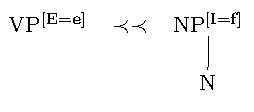
\includegraphics[scale=1]{NaTemp.pdf}
\begin{tikzpicture}[baseline]
\node at (0,0) (VP) {VP\textsuperscript{[E=\textbf{e}]}};
\node (follows) [right = 1em of VP] {$\prec\prec$};
\node [right = 1em of follows] (NP) {NP\textsuperscript{[I=\textbf{f}]}};
\node [below=\baselineskip of NP] (N) {N};
\draw (NP) -- (N);
\end{tikzpicture}
\end{minipage}
\caption{Time scale constructor: case of a scale with one marked point \label{constructor:time}}
\end{figure}

\begin{figure}
% \begin{minipage}{0.2\textwidth}
\avm{
\btag{f} [\type*{hurricane}
	   \TIME & \1\\
	   \LOC & \2\\
	   \NAME & \3
]
}
% \end{minipage}
\hfill%
% \begin{minipage}{0.55\textwidth}
\avm{
\btag{e} [\type*{event}
	\NOUNDIM & [ \type*{time $\und$ one-point-scale}
			\MARKED & \1
	 ]
]
}
% \end{minipage}
\hfill%
% \begin{minipage}{0.2\textwidth}
\avm{
\btag{f} [\type*{hurricane}
	   \TIME & \1\\
	   \LOC & \2\\
	   \NAME & \3
]
}
% \end{minipage}
\caption{Frame representations of the noun \textit{uragan} `hurricane': dictionary entry on the left and the result of the unification with the time scale constructor on the right \label{frame:hurricane}}
\end{figure}

If the enriched noun representation is combined with the representation of the verb \textit{pere\v{z}it'} `to outlive', the resulting frame describes a bounded process of living of the (yet unspecified) actor that started before the hurricane time and ended after it. This frame is shown on \figref{frame:outlive:hurricane}. As in the case of crossing the road, the hurricane is not an argument of the verb and the two frames are only connected via the identity of the values of the attributes \NOUNDIM.

\begin{figure}
\begin{minipage}{0.7\textwidth}\centering
\avm{
\btag{e} [\type*{\isi{bounded-event} $\und$ process $\und$} \type*{proper-scale $\und$ \isi{one-marked-point} $\und$ time}
	\MANN & [\type*{live}]\relax\\
    \ACTOR & \tag{0}\\
    \VERBDIM & \btag{e}\\
  	\NOUNDIM & \btag{e}\\
    \MARKED & \2\\
    \INIT & [\type*{stage}
       \POS & \1 ]\\
     \FIN & [\type*{stage}
       \POS & \3 ]\\
  ]
}
\end{minipage}\hfill%
\begin{minipage}{0.3\textwidth}\centering
\avm{
\btag{f} [\type*{hurricane}
	   \TIME & \2\\
	   \LOC & \5\\
	   \NAME & \6\\
]
}\\
\svar{1} $<$ \svar{2} $<$ \svar{3}\\
\end{minipage}
\caption{Frame representation of the verbal phrase \textit{pere\v{z}it' uragan} `to survive the hurricane': dictionary entry on the left and enriched representation on the right \label{frame:outlive:hurricane}}
\end{figure}

The extraction of the marked point on the \isi{time scale} can be also performed with nouns that lack explicit time points, such as person names like \textit{Ma\v{s}a} `Masha'. Of course, such extraction requires a more complex procedure that cannot be described in detail here, but the idea is that some significant point related to the event type denoted by the verb is extracted using a special constructor. In case of the event of living and a person \textit{Ma\v{s}a} `Masha' this point should be the time of Masha's death. To obtain is, one can use the constructor that creates a representation of the event of living of Masha from the representation of the name \textit{Ma\v{s}a} (using the representation of the \isi{derivational base} for the \Prefix{pere-}prefixed verb, so in our case the frame on \figref{frame:live}). The tentative result of an application of such a constructor is shown on \figref{frame:Masha:live}.

\begin{figure}
\centering
\avm{
\btag{e} [\type*{process}
    \MANN & [\type*{live}]\\
    \ACTOR & [\type*{Masha}]\\
    \NOUNDIM & [\type*{time}
		\MARKED & \2    
    ]\\
    \VERBDIM & \btag{e}\\
    \MDIM & \btag{e}\\
    \MIN & \1\\
    \MAX & \2
  ]
}
\caption{Frame representation of the referent of the name \textit{Ma\v{s}a}, coerced into event interpretation using the verb \textit{\v{z}it'} `to live' \label{frame:Masha:live}}
\end{figure}

Now let us combine the \isi{frame representation} of the verb \textit{pere\v{z}it'} `to outlive' and the representation of \textit{Ma\v{s}a} interpreted as an event of living of Masha that provides as a marked point Masha's time of death. Let us also fill the \ACTOR slot with the referent of the name \textit{Vasya}. With this, we obtain the \isi{frame representation} of the tenseless variant of the phrases \textit{Vasja pere\v{z}il/pere\v{z}iv\"{e}t Ma\v{s}u} `Vasya outlived/will outlive Masha'. This representation is provided on \figref{frame:Vasja:outlive:Masha} and contains the following information: the sentence describes a bounded event \btag{e} of living of Vasya. There is another event \btag{f} of living of Masha, that is not central but is used for the \isi{comparison}. The main event \btag{e} started at the time prior to the \isi{maximum point} of living of Masha (point of Masha's death) and ended or will end at the time after the time of Masha's death. The relation between the time of Vasya's life and the time of Masha's birth is not specified.

\begin{figure}
\begin{minipage}{0.6\textwidth}
\avm{
\btag{e} [\type*{\isi{bounded-event} $\und$ process $\und$} \type*{proper-scale $\und$ one-marked-point}
	\MANN & [\type*{live}]\\
    \ACTOR & [\type*{Vasya}]\\
    \VERBDIM & \btag{e}\\
  	\NOUNDIM & \btag{e}\\
    \MARKED & \2\\
    \INIT & [\type*{stage}
       \POS & \1 ]\\
     \FIN & [\type*{stage}
       \POS & \3 ]\\
  ]
}
\end{minipage}\hfill%
\begin{minipage}{0.35\textwidth}\centering
\avm{
  \btag{f} [\type*{process}
    \MANN & [\type*{live}]\\
    \ACTOR & [\type*{Masha}]\\
    \NOUNDIM & \btag{e}\\
    \VERBDIM & \btag{e}\\
    \MDIM & \btag{e}\\
    \MIN & \5\\
    \MAX & \2
  ]
}\\
\svar{1} $<$ \svar{2} $<$ \svar{3}
\end{minipage}
\caption{Frame representation of the tenseless variant of the phrases \textit{Vasja pere\v{z}il/pere\v{z}iv\"{e}t Ma\v{s}u} `Vasya outlived/will outlive Masha'  \label{frame:Vasja:outlive:Masha}}
\end{figure}

To complete the picture, let us consider the verb \textit{igrat'} `to play'. This verb does not provide a preselected \isi{measure dimension}, so there is some freedom with respect to the selection of a relevant parameter of the direct object. The frame for the verb \textit{igrat'} `to play' is shown on the left side of \figref{frame:outplay}. 

When the representation of the verb \textit{igrat'} is combined with the representation of the prefix \Prefix{pere-} that is compatible with a marked point  scale, we obtain the frame shown on the right side of \figref{frame:outplay} that represents the semantics of the verb \textit{pereigrat'} `to outplay': a bounded event of \MANN \textit{play} that ends at a point of the scale above the marked point. 

The type of the scale and the marked point remain underspecified and need to be identified using the information about the direct object. I propose to use the same strategy as above: if the direct object is a referent of the name \textit{Ma\v{s}a}, the dimension constructor is based on the frame for the verb \textit{igrat'} `to play' to obtain an event of Masha playing that has some parameters, such as \isi{duration} of the play or the quality of the play. As we have discussed in Section~\ref{subsection:semantics:pere}, such sentences as \textit{Vasja pereigral Ma\v{s}u} `Vasya outplayed Masha' are ambiguous and hard to interpret without the \isi{context} that would provide the relevant parameter. The representations that can be obtained as a result of such complex scale extraction procedure are shown on \figref{frame:Masha:play}: the time-related interpretation on the left side and the quality-related interpretation on the right side.

\begin{figure}\small
\begin{minipage}{0.3\textwidth}
\avm{
\btag{e} [\type*{activity}
    \MANN & [\type*{play}]\\
    \ACTOR & \1\\
    \VERBDIM & \btag{e}
  ]
}
\end{minipage}\hfill%
\begin{minipage}{0.65\textwidth}\centering
\avm{
\btag{e} [\type*{\isi{bounded-event} $\und$ activity}
  	\NOUNDIM & \4\\
  	\MANN & [\type*{play}]\\
    \ACTOR & \6\\
    \VERBDIM & \btag{e}\\
    \MDIM & \4 [
       \type*{proper-scale $\und$ one-marked-point}
       \MARKED & \2 ]\\
    \INIT & [\type*{stage}
       \POS & \1 ]\\
     \FIN & [\type*{stage}
       \POS & \3 ]\\
  ]
}\\
\svar{1} $<$ \svar{2} $<$ \svar{3}
\end{minipage}
\caption{Frame representations of the verbs \textit{igrat'} `to play' (left) and \textit{pereigrat'} `to outplay' (right) \label{frame:outplay}}
\end{figure}

\begin{figure}
\begin{minipage}{0.45\textwidth}
\avm{
\btag{e} [\type*{activity}
    \NOUNDIM & [\type*{time}
		\MARKED & \2    
    ]  ]
}\\

\avm{
\btag{f} [\type*{activity}
    \MANN & [\type*{play}]\\
    \ACTOR & [\type*{Masha}]\\
    \VERBDIM & \btag{f}\\
    \DURATION & \2\\
    \QUALITY & \3
  ]
}\\
\end{minipage}
\hfill
\begin{minipage}{0.45\textwidth}
\avm{
\btag{e} [\type*{activity}
    \NOUNDIM & [\type*{quality}
		\MARKED & \3    
    ]
  ]
}\\
\avm{
\btag{f} [\type*{activity}
    \MANN & [\type*{play}]\\
    \ACTOR & [\type*{Masha}]\\
    \VERBDIM & \btag{f}\\
    \DURATION & \2\\
    \QUALITY & \3
  ]
}
\end{minipage}
\caption{Frame representations of the referent of the name \textit{Ma\v{s}a}, coerced into event interpretation using the verb \textit{igrat'} `to play' and then enriched with measure dimension information \label{frame:Masha:play}}
\end{figure}

On the last step one of these representations gets combined with the frame for the verb \textit{pereigrat'} `to outplay' (let us take the quality interpretation) and the resulting frame denotes an event of playing by some \ACTOR  where the end of the playing event is associated with a higher value on the quality scale than the marked point that is the quality of Masha's playing.

\begin{figure}
\begin{minipage}{0.55\textwidth}
\avm{
\btag{e} [\type*{\isi{bounded-event} $\und$ activity}
  	\NOUNDIM & \4\\
  	\MANN & [\type*{play}]\\
    \ACTOR & \6\\
    \VERBDIM & \btag{e}\\
    \MDIM & \4 [
       \type*{proper-scale $\und$} \type*{one-marked-point} \type*{$\und$ quality}
       \MARKED & \2 ]\\
    \INIT & [\type*{stage}
       \POS & \1 ]\\
     \FIN & [\type*{stage}
       \POS & \3 ]\\
  ]
}
\end{minipage}\hfill%
\begin{minipage}{0.4\textwidth}\centering
\avm{
\btag{f} [\type*{activity}
    \MANN & [\type*{play}]\\
    \ACTOR & [\type*{Masha}]\\
    \VERBDIM & \btag{f}\\
    \DURATION & \5\\
    \QUALITY & \2
  ]
}\\
\svar{1} $<$ \svar{2} $<$ \svar{3}
\end{minipage}
\caption{Frame representation of the verbal phrase \textit{pereigrat' Ma\v{s}u} `to outplay Masha' \label{frame:outplay:Masha}}
\end{figure}

\subsection{Iterative interpretation}
The last usage of the prefix \Prefix{pere-} that I provide a frame for is iterative and arises when the \isi{measure dimension} of the event denoted by the \isi{derivational base} is of type \textit{property-scale}. This event then becomes a value of the \isi{preparatory phase} attribute of the new event. The initial and the final stages, the noun dimension, the \isi{measure dimension}, and the manner attributes are copied to the event node that refers to the new event. 

\begin{figure}
\begin{minipage}{0.5\textwidth}
\avm{
\btag{f}  [\type*{bounded-event}
     \MDIM & \3 [\type*{property-scale} ]\\
     \NOUNDIM & \4\\
     \INIT &  \1\\
     \FIN &  \2 \\
     \MANN & \5\\
     \PREP & \btag{e} [\type*{event}
  	 	\THEME & \6\\
        \MDIM & \3\\
    	\NOUNDIM & \4\\
    	\INIT &  \1\\
     	\FIN &  \2 \\
     	\MANN & \5
     ]
  ]
 }
 \end{minipage}\hfill%
 \begin{minipage}{0.45\textwidth}
% %  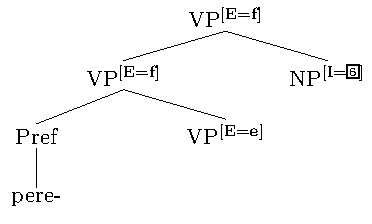
\includegraphics[scale=.85]{PereV.pdf}
\begin{forest}
[VP\textsuperscript{[E=\textbf{f}]}
 [VP\textsuperscript{[E=\textbf{f}]}
   [Pref [\Prefix{pere-}]]
   [VP\textsuperscript{[E=\textbf{e}]}]
 ] [NP\textsuperscript{[I=\avm{\6}]}]
]
\end{forest}
 \end{minipage}
\caption{Representation of the contribution of the prefix \Prefix{pere-}: case of a property scale \label{frame:pere:iter}}
\end{figure}

The next restriction, apart from the property type of the scale, is that the event denoted by the \isi{derivational base} must have a final stage in its representation. This means that a simplex imperfective verb cannot be combined with this prefix usage, unless it is \isi{coerced into} a bounded event. On the formal side it means that we need a way to formulate the requirement on the frame (presence of the \FIN attribute). For implementing the coercion of an unbounded event into a bounded event I propose to use the frame shown on \figref{frame:coerce}. On the syntactic side it is accompanied by the introduction of an extra VP node.

\begin{figure}
% \begin{minipage}{0.7\textwidth}
\hfill%
\avm{
\btag{e}  [\type*{bounded-event}
     \MDIM & \3 [\type*{\isi{property-scale} $\und$ closed-scale} 
		\MIN & \1\\
		\MAX & \2      
      ]\\
     \NOUNDIM & \3\\
     \INIT &  [\type*{stage}
     	\POS & \1]\\
     \FIN &  [\type*{stage}
     	\POS & \2]\\
  ]
 }\hfill%
%  \end{minipage}
%  \begin{minipage}{0.25\textwidth}
% %  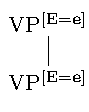
\includegraphics[scale=1]{VPcoerce.pdf}\hfill
\begin{forest}
[VP\textsuperscript{[E=\textbf{e}]}
  [VP\textsuperscript{[E=\textbf{e}]}]
]
\end{forest}
%  \end{minipage}
\caption{Frame and tree for coercion of an unbounded event into a bounded event \label{frame:coerce}}
\end{figure}

\begin{figure}
\centering
\avm{
\btag{e} [\type*{\isi{bounded-event} $\und$ activity}
	\MANN & [\type*{play}]\\ 
	\ACTOR & \4\\
    \VERBDIM & \btag{e}\\
     \MDIM & \3 [\type*{\isi{property-scale} $\und$ closed-scale} 
		\MIN & \1\\
		\MAX & \2      
      ]\\
     \NOUNDIM & \3\\
     \INIT &  [\type*{stage}
     	\POS & \1]\\
     \FIN &  [\type*{stage}
     	\POS & \2]\\
  ]
}
\caption{Frame of the verb \textit{igrat'} `to play', coerced into a bounded event interpretation \label{frame:igrat:coerce}}
\end{figure}

Now if we take an imperfective verb, such as \textit{igrat'} `to play', and first coerce it using the frame on \figref{frame:coerce} (this operation is performed in the \isi{metagrammar} and its result is shown on \figref{frame:igrat:coerce}) and then attach the prefix \Prefix{pere-} with the semantic representation shown on \figref{frame:pere:iter}, we obtain the frame shown on \figref{frame:pere:igrat}. This frame describes a bounded event of manner \textit{play} that is measured along the property scale, the initial stage being located at the \isi{minimum of the scale} and the final stage being located at the maximum of the scale. In addition, there is a \isi{preparatory phase} that refers to another event with similar characteristics.

\begin{figure}
\centering
\avm{
\btag{f} [\type*{bounded-event}
  		 \ACTOR & \4\\
  		 \THEME & \7\\
     	\MDIM & \3  [\type*{\isi{property-scale} $\und$ closed-scale} 
			\MIN & \1\\
			\MAX & \2      
      	]\\
     	\NOUNDIM & \3\\
     	\INIT &  [\type*{stage}
     		\POS & \1
     	]\\
     	\FIN &  [\type*{stage}
     		\POS & \2
     	]\\
     	\MANN & [\type*{play}]\\
     	\PREP & \btag{e}  [\type*{bounded-event}
     		\ACTOR & \6\\
     		\THEME & \7\\
     		\MDIM & \3\\
     		\NOUNDIM & \3\\
      		\MANN & [\type*{play}]\\
     		\INIT &  [\type*{stage}
     			\POS & \1
     		]\\
     		\FIN &  [\type*{stage}
     			\POS & \2
     		]\\
    		\VERBDIM & \btag{e}
  		]
  ]
 }
\caption{Frame representation of the verb \textit{pereigrat'} `to replay' \label{frame:pere:igrat}}
\end{figure}

When the verb \textit{pereigrat'} `to replay' is used, an appropriate noun, probably unified with some dimension constructor, should occupy the position of the theme and contribute additional information about the scale. Let us take the noun \textit{partija} `match' that is probably characterized by \isi{duration}, the type of the game it is a match of, and the set of players (see the left side of \figref{frame:match}). We are interested in particular in the \DURATION attribute as it is the only parameter that can bind the event. As we have already seen before, this attribute can be used to enrich the representation with the \isi{measure dimension} information, as shown on \figref{frame:match}.

\begin{figure}\small
% \begin{minipage}{0.4\textwidth}
\avm{
\btag{g} [\type*{match}
	   \DURATION & \1\\
	   \GAME & [\type*{game}]\\
	   \PLAYERS & [\type*{entity}
	   		\CARD & \2
	   ] 
]
}\hfill%
% \end{minipage}
% \begin{minipage}{0.55\textwidth}
\avm{
\btag{f}[\type*{event}
 \NOUNDIM & [ \type*{time $\und$ closed-scale} \type*{$\und$ measure-of-change}
			\MIN & 0\\
			\MAX & \1
	   ]
]
}
% \end{minipage}
\caption{Frame representations of the noun \textit{partija} `match' (left) and of an additional component that is obtained as a result of its unification with the dimension constructor (right) \label{frame:match}}
\end{figure}

As a final step, we can now combine the frames on Figures~\ref{frame:pere:igrat} and~\ref{frame:match} and obtain the frame shown on \figref{frame:pere:igrat:match}. This frame describes a bounded event of playing that is preceded with another such event and both events are measured out according to the \isi{duration} of the match. 

\begin{figure}\small
\avm{
\btag{f} [\type*{bounded-event}
  		 \ACTOR & \4\\
     	\MDIM & \3  [\type*{\isi{property-scale} $\und$ \isi{closed-scale} $\und$ time $\und$ measure-of-change} 
			\MIN & 0\\
			\MAX & \2   
      	]\\
     	\NOUNDIM & \3\\
     	\INIT &  [\type*{stage}
     		\POS & \1
     	]\\
     	\FIN &  [\type*{stage}
     		\POS & \2
     	]\\
     	\MANN & [\type*{play}]\\
     	\PREP & \btag{e} [\type*{bounded-event}
     		\ACTOR & \6\\
     		\THEME & \btag{g} [\type*{match}
	   			\DURATION & \2\\
	   			\GAME & [\type*{game}]\\
	   			\PLAYERS & [\type*{entity}
	   				\CARD & \7
	   			]
	   		]\\
     		\MDIM & \3\\
     		\NOUNDIM & \3\\
      		\MANN & [\type*{play}]\\
     		\INIT &  [\type*{stage}
     			\POS & \1
     		]\\
     		\FIN &  [\type*{stage}
     			\POS & \2
     		]\\
    		\VERBDIM & \btag{e}
  		]
  ]
 }
\caption{Frame representation of the verbal phrase \textit{pereigrat' partiju} `to replay the match' \label{frame:pere:igrat:match}}
\end{figure}

\clearpage

\section{Frame semantics for the prefix \textit{do-}}\label{section:frame:do}
The last prefix I will provide a frame for is the prefix \Prefix{do-}. As we have discussed in Chapter~\ref{Chapter5}, primarily following \citet{Kagan:book}, this prefix has \isi{completive} or additive semantics: it can refer to the terminal part of the event or an event that can be seen as a continuation of another event. In Section~\ref{subsection:semantics:do} I came to the following conclusions with respect to the selection of the scale for the \isi{measure dimension}: the first choice is the pre-specified verbal scale, next comes the scale extracted from the representation of the noun, and the last option is the event scale. 

This scheme can be realised by identifying the values of the \isi{measure dimension} and the noun dimension attributes and adding an extra rule that would equate the \isi{verbal dimension} with the \isi{measure dimension} for intransitive verbs. When the prefix is attached, the maximum of the scale has to be associated with the final stage of the event. The frame that realises these ideas is shown on \figref{frame:do}. Note that attributes in Frame Semantics are functional, so the attribute \PARTOF has to satisfy this restriction as well. To ensure this, I propose to define the value of this attribute as  the maximum event that the event in question is part of. In particular, it would be an event that proceeds from the minimum to the maximum degree on the relevant scale (provided by the \MDIM attribute). The scale has to be closed in order for the value of the \PARTOF attribute to be defined.

\begin{figure}
\begin{minipage}{0.45\textwidth}
\avm{
\btag{f} [\type*{bounded-event}
   		\MANN & \4\\
   		\ACTOR & \5\\
  	 	\THEME & \9\\
        \MDIM & [ \type*{\isi{closed-scale} $\und$} \type*{property-scale}
			\MIN & \2\\
			\MAX & \1						
        ]\\
    	\INIT & [\type*{stage}
    		\POS &  \3]\\
     	\FIN &  [\type*{stage}
    		\POS &  \1]\\
     	\PARTOF & \btag{e}\\
       \NOUNDIM & [\7]\\
       \VERBDIM & [\8]
    ]
 }
 \end{minipage}\hfill%
 \begin{minipage}{0.45\textwidth}\centering
\avm{
\btag{e} [\type*{bounded-event}
   		\MANN & \4\\
   		\ACTOR & \6\\
  	 	\THEME & \9\\
        \MDIM & [ \type*{\isi{closed-scale} $\und$} \type*{property-scale}
			\MAX & \1						
        ]\\
    	\INIT &  [\type*{stage}
    		\POS &  \2]\\
     	\FIN &  [\type*{stage}
    		\POS &  \1]\\
       \NOUNDIM & [\7]\\
       \VERBDIM & [\8]
    ]
 }\\
$\tuple{\btag{f}\BC\MDIM,\btag{e}\BC\MDIM}\D\type{segm-of}$\\[1ex]
\end{minipage}
\caption{Frame representation of the prefix \Prefix{do-} \label{frame:do}}
\end{figure}

Similarly to the iterative usage of the prefix \Prefix{pere-}, the prefix \Prefix{do-} can be only attached to \isi{bounded events}. This means that, again, simplex \isi{imperfective verbs} need to be first \isi{coerced into} a bounded interpretation. For coercion I propose to use the same frame as we have used before when combining the verbs with the prefix \Prefix{pere-}: coercion frame shown on \figref{frame:coerce}. As we have already performed coercion for the verb \textit{igrat'} `to play', let us see how the prefix \Prefix{do-} attaches to this verb. For this, we take the frame on \figref{frame:do} and use the frame on \figref{frame:igrat:coerce} as a base event identified as \btag{e} in the frame on \figref{frame:do}. As a result we obtain the frame shown on \figref{frame:do:igrat} that refers to a bounded event that is part of another event. The scale of the new event is also a part of the scale of the event denoted by the \isi{derivational base}. 

\begin{figure}\small
 \begin{minipage}{0.45\textwidth}
\avm{
\btag{f} [\type*{bounded-event}
   		\MANN & \4\\
   		\ACTOR & \5\\
  	 	\THEME & \8\\
        \MDIM & [\type*{property-scale} \type*{$\und$ closed-scale} 
			\MIN & \2\\
			\MAX & \1						
        ]\\
    	\INIT &  [\type*{stage}
    		\POS &  \3]\\
     	\FIN &  [\type*{stage}
    		\POS &  \1]\\
     	\PARTOF & \btag{e}\\
       \NOUNDIM & [\type*{property-scale} \type*{$\und$ closed-scale}]\\
       \VERBDIM & [\type*{bounded-event} \type*{$\und$ activity}]
    ]
 }
 \end{minipage}\hfill%
  \begin{minipage}{0.45\textwidth}\centering
 \avm{
\btag{e} [\type*{bounded-event} \type*{$\und$ activity}
	\MANN & [\type*{play}]\\ 
	\ACTOR & \6\\
  	 \THEME & \8\\
    \VERBDIM & \btag{e}\\
     \MDIM & \3 [\type*{property-scale} \type*{$\und$ closed-scale} 
		\MIN & \2\\
		\MAX & \1      
      ]\\
     \NOUNDIM & \3\\
     \INIT &  [\type*{stage}
     	\POS & \2]\\
     \FIN &  [\type*{stage}
     	\POS & \1]\\
  ]
}\\
$\tuple{\btag{f}\BC\MDIM,\btag{e}\BC\MDIM}\D\type{segm-of}$\\[1ex]
\end{minipage}
\caption{Frame representation of the verb \textit{doigrat'} `to finish playing' \label{frame:do:igrat}}
\end{figure}

To make clear why the complicated rules of how the \isi{measure dimension} is constructed are needed, let me show what happens when the direct object comes into play and how the verb prefixed with \Prefix{do-} once differs from the verb prefixed with the same prefix twice. The frame on \figref{frame:do:igrat:partiju} shows the representation of the phrase \textit{doigrat' partiju} `to finish playing the match', formed using the frame on \figref{frame:do:igrat} and the frame on the right side of \figref{frame:match}. It is important to note that the information that comes from the direct object is unified at the deepest relevant level: this means that for a non-suffixed verb with multi-event representation it would be always the representation of the event denoted by the base verb. In case of the prefix \Prefix{pere-}, despite the multi-layer representation, this did not play a role, as all the information is passed to the higher layer without changes. Here, however, the \THEME is identical for the partial event and the whole event, but the noun dimension of the new event only inherits the type of the scale and not the values of the extreme points. Instead, a new scale of the same type, but probably with a different \MIN point, is constructed.

\begin{figure}\small
\avm{
\btag{e} [\type*{bounded-event}
   		\MANN & \7 [\type*{play}]\\
   		\ACTOR & \5\\
  	    \THEME & \8\\
        \MDIM & [\type*{\isi{property-scale} $\und$ closed-scale} 
			\MIN & \2\\			
			\MAX & \1						
        ]\\
    	\INIT &  [\type*{stage}
    		\POS &  \3]\\
     	\FIN &  \6\\
     	\PARTOF & \btag{e}\\
       \NOUNDIM & [\type*{\isi{property-scale} $\und$ closed-scale}]\\
       \VERBDIM & [\type*{\isi{bounded-event} $\und$ activity}]
    ]
 }\medskip\\
 \avm{
\btag{e} [\type*{\isi{bounded-event} $\und$ activity}
	\MANN & \7\\ 
  	 \THEME & \8[\type*{match}
	   \DURATION & \1\\
	   \GAME & [\type*{game}]\\
	   \PLAYERS & [\type*{entity}
	   		\CARD & \2
	   ]\\
	   \NOUNDIM & \3
	]\\
	\ACTOR & \9\\
    \VERBDIM & \btag{e}\\
     \MDIM & \3 [\type*{time $\und$ measure-of-change $\und$ \isi{property-scale} $\und$ closed-scale} 
		\MIN & 0\\
		\MAX & \1     
      ]\\
     \NOUNDIM & \3\\
     \INIT &  [\type*{stage}
     	\POS & \2]\\
     \FIN &  \6 [\type*{stage}
     	\POS & \1]\\
  ]
}\\
$\tuple{\btag{f}\BC\MDIM,\btag{e}\BC\MDIM}\D\type{segm-of}$\\[1ex]
\caption{Frame representation of the verbal phrase \textit{doigrat' partiju} `to finish playing the match' \label{frame:do:igrat:partiju}}
\end{figure}

As one can see on \figref{frame:do:igrat:partiju}, in this case the \isi{measure dimension} of the partial event is the same as the \isi{measure dimension} of the whole event. It is different when two prefixes are stacked, as in the verb \textit{dodoigrat'} `to finish playing the final part'. One would like to see a different semantic representation in this case, while otherwise such verb could not be used, as it would violate the pragmatic principles. Under the analysis I propose here, the verbal phrase \textit{dodoigrat' partiju} `to finish playing the final part of the match' receives the \isi{frame representation} shown on \figref{frame:do:do:igrat:partiju} (this frames makes reference to the frame shown on \figref{frame:do:igrat:partiju}). So the event denoted by the verbal phrase \textit{dodoigrat' partiju} `to finish playing the final part of the match' is an event of playing that does not necessarily start from the \isi{minimum of the scale} and the \isi{minimum of the scale} is not bound to the beginning of the match. Such a frame still allows the interpretation that the new event refers to an event of playing the whole match, but this will be blocked by pragmatic reasoning.

\begin{figure}
\avm{
\btag{g} [\type*{bounded-event}
   		\MANN & \7 [\type*{play}]\\
   		\ACTOR & \4\\
  	    \THEME & \8\\
        \MDIM & [\type*{time $\und$ measure-of-change $\und$ \isi{property-scale} $\und$ closed-scale} 
			\MIN & \3\\			
			\MAX & \1						
        ]\\
    	\INIT &  [\type*{stage}
    		\POS &  \tag{10}]\\
     	\FIN &  \6 [\type*{stage}
    		\POS &  \1]\\\\
     	\PARTOF & \btag{f}\\
       \NOUNDIM & [\type*{\isi{property-scale} $\und$ closed-scale}]\\
       \VERBDIM & [\type*{\isi{bounded-event} $\und$ activity}]
    ]
 }\\
$\tuple{\btag{g}\BC\MDIM,\btag{f}\BC\MDIM}\D\type{segm-of}$\\[1ex]
\caption{Frame representation of the verbal phrase \textit{dodoigrat' partiju} `to finish playing the final part of the match': additional component with respect to \figref{frame:do:igrat:partiju} \label{frame:do:do:igrat:partiju}}
\end{figure}

Let me show what happens when the prefix \Prefix{do-} is attached to a verb that has a pre-selected \isi{measure dimension}. Consider a determinate \isi{motion verb} \textit{be\v{z}at'} `to run' that we have used earlier in combination with the prefix \Prefix{pere-} (see \figref{frame:bezhat}). The basic verb \textit{be\v{z}at'} `to run' also has to be coerced before \isi{prefixation}, so instead of doing this step (that would be similar to the procedure above, illustrated by the verb \textit{igrat'} `to play'), let us take as an input the prefixed verb \textit{perebe\v{z}at'} `\isi{to cross}'. The result of combining the \isi{frame representation} of the verb \textit{perebe\v{z}at'} `\isi{to cross}' (right side of \figref{frame:bezhat}) with the \isi{frame representation} of the prefix \Prefix{do-}, shown on \figref{frame:do}, is provided on \figref{frame:do:perebezhat}. This verb denotes an event that is a part of an event of crossing the road and necessarily includes the final part of the crossing. 

\begin{figure}
\begin{center}
\avm{
\btag{f} [\type*{\isi{bounded-event} $\und$ transloc}
   		\MANN & [\type*{run}]\\
   		\ACTOR & \5\\
        \MDIM & \7 [ \type*{path $\und$ \isi{closed-scale} $\und$ proper-scale}
			\MIN & \2\\
			\MAX & \1						
        ]\\
    	\INIT &  [\type*{stage}
       		\POS & \3 ]\\
     	\FIN &  \8 \\
     	\PARTOF & \tag{0}\\
       \NOUNDIM & \7\\
       \VERBDIM & \7 [ \type*{path $\und$ \isi{closed-scale} $\und$ property-scale}]
    ]
 }\\
 \vspace{1em}
\avm{
\btag{e} [\type*{\isi{bounded-event} $\und$ transloc}
	   	\MANN & [ \type*{run} ]\\
       	\ACTOR & \6\\
	   \PATH & [\type*{path}]\\
	   	\TRACE & [ \type*{trace} ]\\
	   	\VERBDIM & \4 \\
	   	\MDIM & \4 [ \type*{path $\und$ \isi{closed-scale} $\und$ proper-scale}
       		\MIN & \9\\
       		\MAX & \1
       	]\\
      	\NOUNDIM & \4\\
    	\INIT & [\type*{stage}
       		\POS & \9 ]\\
     	\FIN & \8 [\type*{stage}
       		\POS & \1 ]
    ]
 }\\
 $\tuple{\btag{f}\BC\MDIM,\btag{e}\BC\MDIM}\D\type{segm-of}$\\[1ex]
 \end{center}
\caption{Frame representation of the verb \textit{doperebe\v{z}at'} `to finish crossing' \label{frame:do:perebezhat}}
\end{figure}

%\section{Semantics for the imperfective suffix}
%\section{Compositional semantics}
%\section{Testing the predictions}
%
%
%
%\section{Metagrammar}
%Linguistic generalizations in TAGs are captured by a \isi{metagrammar}. There are two steps of factorization, which are important for this paper:
%\begin{itemize}
%\renewcommand{\labelitemi}{$\bullet$}
%\item \textit{unanchored elementary trees} are specified separately from \isi{lexical anchors};
%\item trees are organized into \textit{tree families} which represent different realizations of one subcategorization frame.
%\end{itemize}
%This allows to define a meaning for sets of unanchored elementary trees, i.e., a meaning of constructions.
%
%\section{Morphological decomposition}\label{sec-morph}
%\section{Inducing aspectual properties from semantic representation}
%
%How to make sure we get the appropriate object: 
%As suggested by \citet{Rappaport:08}, ``\isi{scales} require that the participant whose property is measured by them be overtly realized." I want to slightly modify this suggestion and claim that whenever a point on the scale is used to determine when the event terminates, this point cannot be related to an unbound variable. If no link between such point and the world has been specified, the whole derivation fails. 

\section{Summary}
In this chapter I have proposed frame representations of the semantic contribution of five Russian verbal prefixes: \Prefix{za-}, \Prefix{na-}, \Prefix{po-}, \Prefix{pere-}, and \Prefix{do-}. We have seen that these representations are quite distinct: in case of the prefix \Prefix{za-} the derived verb refers to a transition that is connected with the event denoted by the \isi{derivational base} via relations; the prefixes \Prefix{na-} and \Prefix{po-} both add information to the initial event frame, but differ with respect to the processes of dimension selection and assigning scale degrees to the initial and final stages of the event; the prefix \Prefix{pere-} creates a new event with a \isi{preparatory phase} consisting of the event denoted by the \isi{derivational base}; and the prefix \Prefix{do-} refers to a partial event that is constructed during the derivation with a probable change of the minimum point of the \isi{measure dimension} scale.

We have also seen that in order to obtain the representation of the derived verb, several steps related to the scalar selection process have to be made. We need to select the dimension of the verb, the relevant dimension of the object, and find out the type of the scale that will be used for measuring the event. In some cases this scale is the event itself. 

As objects are often associated with different dimensions, I have proposed various constructors that allow to extract relevant information. Some of these constructors (e.g., \isi{temperature dimension} constructor, \figref{constructor:temp}) can be applied without restrictions, some (e.g., \isi{amount dimension} constructor, \figref{constructor:amount}) are accompanied by \isi{syntactic restrictions}, and some (e.g., the constructor that reconstructs the event of living from the person's name) can be used only in special cases when the scalar interpretation is required and no other constructor can be applied. As modelling semantic representation and shifts of meaning of nouns is not the goal of this work, the proposed constructors will most probably require revisions, but they suffice to illustrate how the object can contribute to determining the interpretation of the prefixed verb.

The representations I have proposed here differ in their complexity: while frames for some prefixed verbs differ from the representations of the respective derivational bases only by the presence of several additional attributes (as in case of the prefixes \Prefix{po-} and \Prefix{na-}), frames for other prefixed verbs are a lot more complex (prefixes \Prefix{do-} and \Prefix{pere-}). A hypothesis that would be interesting to check empirically is whether in case of verbs that are represented using multi-layered frames the interpretation requires an increased amount of processing time relative to verbs with the same \isi{morphological complexity} but less complex semantic representation.


In the next part, Chapter~\ref{Chapter8}, I will show how frame representations proposed in this chapter can be implemented using a \isi{metagrammar} compiler.
